\documentclass{article}
\usepackage[brazil]{babel}
\usepackage[utf8]{inputenc}
\usepackage[T1]{fontenc}
\usepackage{lmodern}
\usepackage{soulutf8} 
\setlength{\headheight}{14.5pt}
\usepackage[a4paper,left=2.0cm,right=1.0cm,top=\dimexpr15mm+1.5\baselineskip,bottom=2cm]{geometry}
\usepackage{amsmath}
\usepackage{tikz}
\usepackage{mathdots}
\usepackage{yhmath}
\usepackage{cancel}
\usepackage{color}
\usepackage{wasysym}
\usepackage{siunitx}
\usepackage{array}
\usepackage{xargs}
\usepackage{multirow}
\usepackage{amssymb}
\usepackage{tabularx}
\usepackage{extarrows}
\usepackage{xfrac}
\usepackage{booktabs}
\usetikzlibrary{fadings}
\usetikzlibrary{patterns}
\usetikzlibrary{shadows.blur}
\usetikzlibrary{shapes}
\usepackage[utf8]{inputenc}
\usepackage{amsfonts}
\usepackage{amsmath}
\usepackage{multicol}
\usepackage{fancyhdr}
\usepackage{tikz, tkz-euclide}
\usetikzlibrary{patterns}
\usepackage{enumitem}
\usepackage{arcs}
\usepackage{afterpage}
\usepackage{tcolorbox}
\usepackage{multirow}
\usepackage{numprint}
\usepackage{titlesec}
\usepackage{graphicx}
\usepackage{pgfplots}
\pgfplotsset{compat=1.15}
\usetikzlibrary{patterns}
\pgfplotsset{compat=1.15}
\usepackage{mathrsfs}
\usetikzlibrary{calc,arrows,matrix}
\usetikzlibrary{shapes.geometric}
\usetikzlibrary{positioning,quotes}
\definecolor{BLA}{rgb}{0.26666666666666666,0.26666666666666666,0.26666666666666666}
\definecolor{WHI}{rgb}{255,255,255}

\titleformat{\section}[block]{\Large\bfseries\filcenter}{\thesection}{1em}{\ul}
\titleformat{\subsection}{\large\bfseries\filcenter}{\thesubsection}{1em}{}

\newcommand{\limite}[3][x]{\lim\limits_{{#1}\to{#2}}{#3}}

\newcommand{\sgn}{\hspace{2pt}\mathrm{sgn}\hspace{1pt}}

\newcommand{\pint}[1]{\lfloor{#1}\rfloor}

\newcommand{\deriv}[1]{{#1}^{\prime}}
\newcommand{\segderiv}[1]{{#1}^{\prime\prime}}

\newcommand{\integ}[3]{\int\limits_{#1}^{#2}{#3}}

\newcommand{\fimd}[1]{\hspace{2pt}d{#1}}

\newcommand{\multi}[7]{\textbf{({#1})} {#2}
\begin{enumerate}
    \item {#3}
    
    \item {#4}
    
    \item {#5}
    
    \item {#6}
    
    \item {#7}
\end{enumerate}}

\newcommand{\parenth}[1]{\left({#1}\right)}

\newcommand{\opcaoIMG}[2][0.5]{}

\pgfdeclarepatternformonly{south west lines}{\pgfqpoint{-0pt}{-0pt}}{\pgfqpoint{6pt}{6pt}}{\pgfqpoint{6pt}{6pt}}{
        \pgfsetlinewidth{0.16pt}
        \pgfpathmoveto{\pgfqpoint{0pt}{0pt}}
        \pgfpathlineto{\pgfqpoint{6pt}{6pt}}
        \pgfpathmoveto{\pgfqpoint{5.6pt}{-0.4pt}}
        \pgfpathlineto{\pgfqpoint{6.4pt}{0.4pt}}
        \pgfpathmoveto{\pgfqpoint{-0.4pt}{5.6pt}}
        \pgfpathlineto{\pgfqpoint{0.4pt}{6.4pt}}
        \pgfusepath{stroke}}
        
\makeatletter
\DeclareFontFamily{U}{tipa}{}
\DeclareFontShape{U}{tipa}{m}{n}{<->tipa10}{}
\newcommand{\arc@char}{{\usefont{U}{tipa}{m}{n}\symbol{62}}}%

\newcommand{\arc}[1]{\mathpalette\arc@arc{#1}}

\newcommand{\arc@arc}[2]{
	\sbox0{$\m@th#1#2$}%
	\vbox{
		\hbox{\resizebox{\wd0}{\height}{\arc@char}}
		\nointerlineskip
		\box0
	}%
}
\makeatother

\DeclareFontFamily{U}{skulls}{}
\DeclareFontShape{U}{skulls}{m}{n}{ <-> skull }{}
\newcommand{\skull}{\text{\usefont{U}{skulls}{m}{n}\symbol{'101}}}

\pagestyle{fancy}
\fancyhf{}
\fancyhfoffset[L]{0.5cm} % left extra length
\fancyhfoffset[R]{0.5cm} % right extra length
\lhead{MATH CHRONIC}
\chead{\bfseries 555 problemas de Geometria}
\rhead{Jeferson Almir}
\rfoot{}
\cfoot{\thepage}

\providecommand{\sin}{}
\renewcommand{\sin}{\hspace{2pt}\mathrm{sen}\hspace{1pt}}
\providecommand{\tan}{}
\renewcommand{\tan}{\hspace{2pt}\mathrm{tg}\hspace{1pt}}
\providecommand{\cot}{}
\renewcommand{\cot}{\hspace{2pt}\mathrm{cotg}\hspace{1pt}}
\providecommand{\csc}{}
\renewcommand{\csc}{\hspace{2pt}\mathrm{cossec}\hspace{1pt}}
\providecommand{\arctan}{}
\renewcommand{\arctan}{\hspace{2pt}\mathrm{arctg}\hspace{1pt}}
\providecommand{\arcsin}{}
\renewcommand{\arcsin}{\hspace{2pt}\mathrm{arcsen}\hspace{1pt}}
\newcommand{\arccot}{\hspace{2pt}\mathrm{arccotg}\hspace{1pt}}

\newcommand{\espaco}{$ $}
\newcommand{\dica}{\textbf{Dicas:}}

\newcommand{\iniTri}{Seja $ABC$ um triângulo}

\definecolor{ffqqqq}{rgb}{1.,0.,0.}
\definecolor{qqqqff}{rgb}{0.,0.,1.}
  
  
  
\begin{document}
\begin{center}
Professor: Jeferson Almir
\end{center}

Aluno(a): \underline{\hspace{12cm}}
Nº: \underline{\hspace{2cm}}

Data: \underline{\hspace{2cm}}/\underline{\hspace{2cm}}/\underline{\hspace{2cm}}

\begin{multicols}{2}

\section{Problemas}

\renewcommand{\labelenumi}{\textbf{\arabic{enumi}.}}
\renewcommand\labelenumi{\textbf{\nplpadding{3}\numprint{\arabic{enumi}}.}}

\begin{enumerate}

    \item Seja $ABC$ um triângulo. Prove que suas medianas $CD$, $AE$ e $BF$ são concorrentes. \dica %Áreas %Proporção %Ponto fantasma
    
    \item Seja $ABC$ um triângulo. Prove que suas alturas $AE$, $CF$ e $BD$ são concorrentes. \dica %Quadriláteros cíclicos %Ponto fantasma
    
    \item Prove que as bissetrizes internas de um $\triangle ABC$ são concorrentes. \dica %Definição
    
    \item Seja $ABC$ um triângulo. Seu incírculo toca $AB$, $BC$ e $CA$ nos pontos $C_1$, $A_1$ e $B_1$ respectivamente. Prove que as retas $CC_1$, $BB_1$ e $AA_1$ são concorrentes. \dica %Teorema de Ceva
    
    \item Prove que as mediatrizes dos lados de um dado $\triangle ABC$ são concorrentes. \dica %Definição
    
    \item Seja $ABC$ um triângulo de circuncírculo $k$. Sejam $l_A$, $l_B$ e $l_C$ as retas tangentes a $k$ pelos pontos $A$, $B$ e $C$ respectivamente. Se $l_A\cap l_B=C_1$, $l_B\cap l_C=A_1$ e $l_C\cap l_A=B_1$, prove que as retas $AA_1$, $BB_1$ e $CC_1$ são concorrentes. \dica %Teorema de Ceva %Analise outro triângulo
    
    \item Seja $ABC$ um triângulo. Sejam $A_1$, $B_1$ e $C_1$ os pontos de tangência dos segmentos $BC$, $CA$ e $AB$ com os exincírculos de $\triangle ABC$. Prove que as retas $AA_1$, $BB_1$ e $CC_1$ são concorrentes. \dica %Teorema do Bico %Teorema de Ceva
    
    \item Seja $ABC$ um triângulo e seja $N$ seu ponto de Nagel (ponto de concorrência do exercício anterior). Digamos que $AN$, $BN$ e $CN$ intersectem o incírculo de $\triangle ABC$ nos pontos $A_1$, $B_1$ e $C_1$, e os lados $BC$, $CA$ e $AB$ nos pontos $A_2$, $B_2$ e $C_2$, respectivamente. Prove que $AA_1=NA_2$, $BB_1=NB_2$ e $CC_1=NC_2$. \dica %Ponto fantasma %Tente achar uma homotetia útil %Teorema de Menelaus
    
    \item Seja $ABC$ um triângulo. Os triângulos equiláteros $\triangle ABC_1$, $\triangle AB_1C$ e $\triangle A_1BC$ são construídos no exterior do triângulo $ABC$. Prove que as retas $AA_1$, $BB_1$ e $CC_1$ são concorrentes. \dica %Marque ângulos %Procure quadriláteros cíclicos %Prove colinearidade
    
    \item \iniTri. Os triângulos equiláteros $\triangle ABC_1$, $\triangle AB_1C$ e $\triangle A_1BC$ são construídos no interior do triângulo $ABC$. Prove que as retas $AA_1$, $BB_1$ e $CC_1$ são concorrentes. \dica %Marque ângulos %Procure quadriláteros cíclicos %Prove colinearidade
    
    \item Prove que para um dado $\triangle ABC$, existe algum ponto $X$ tal que vale $AX\cdot BC = BX\cdot AC = CX \cdot AB$. \dica %Círculo de Apolônio %Eixo radical %Teorema de Menelaus
    
    \item Prove que para um dado $\triangle ABC$, exatamente dois pontos satisfazem a condição da questão anterior. \dica %Círculo de Apolônio %Eixo radical %Teorema de Menelaus
    
    \item \iniTri. Prove que existe um ponto único $S$ tal que vale $BC+AS = CA+BS = AB+CS$. \dica %Construa o incírculo do triângulo %Marque medidas %Construa circunferências secantes ao incírculo %Brinque com circunferências tangentes
    
    \item \iniTri. Prove que existe um ponto único $S$ tal que vale $BC-AS = CA-BS = AB-CS$. \dica %Construa o incírculo do triângulo %Marque medidas %Construa circunferências secantes ao incírculo %Brinque com circunferências tangentes %Pense fora da caixa
    
    \item Três circunferências $k_1(A)$, $k_2(B)$ e $k_3(C)$ são dadas, e elas são todas tangentes externamente entre si. Seja $C_1$ e $B_1$ os pontos de tangência de $k_1$ com $k_2$, e de $k_1$ com $k_3$, respectivamente. Seja $A_1$ o ponto de tangência de $k_2$ com $k_3$. A circunferência $k_4$ toca as outras três circunferências externamente. Prove que o primeiro centro de Soddy do $\triangle ABC$ (problema $13$) coincide com o centro de $k_4$. \dica %Faça uma correspondência de construções
    
    \item Três circunferências $k_1(A)$, $k_2(B)$ e $k_3(C)$ são dadas, e elas são todas tangentes externamente entre si. Seja $C_1$ e $B_1$ os pontos de tangência de $k_1$ com $k_2$, e de $k_1$ com $k_3$, respectivamente. Seja $A_1$ o ponto de tangência de $k_2$ com $k_3$. A circunferência $k_4$ toca as outras três circunferências internamente. Prove que o segundo centro de Soddy do $\triangle ABC$ (problema $14$) coincide com o centro de $k_4$. \dica %Faça uma correspondência de construções
    
    \item \iniTri. Sejam $S_1$ e $S_2$ seus primeiro e segundo centros de Soddy (problemas $13$ e $14$), respectivamente. Prove que os pontos $A$, $B$ e $C$ estão sobre uma elipse de focos $S_1$ e $S_2$. \dica %Use a definição desses pontos %Equacione
    
    \item \iniTri. Seja $S_1$ seu primeiro centro de Soddy (problema $13$). Prove que existe uma circunferência inscrita no quadrilátero convexo formado pelas retas $CS_1$, $BS_1$, $AC$ e $AB$. \dica %Construa o incírculo do triângulo %Marque medidas %Construa circunferências secantes ao incírculo %Equacione
    
    \item \iniTri. Seja $S_2$ seu segundo centro de Soddy (problema $14$). Prove que existe uma circunferência que toca as retas $BA$ e $BC$ e os segmentos $AS_2$ e $CS_2$. \dica %Construa o incírculo do triângulo %Marque medidas %Construa circunferências secantes ao incírculo %Tente achar uma versão do Teorema de Pitot para quadriláteros não-convexos %Equacione
    
    \item \iniTri, com exincírculos $\omega_a$, $\omega_b$ e $\omega_c$. Sejam $I_a$, $I_b$ e $I_c$ os centros de $\omega_a$, $\omega_b$ e $\omega_c$ respectivamente. Seja $A_1$ o ponto de tangência de $\omega_a$ com o lado $BC$. Defina os pontos $B_1$ e $C_1$ analogamente. Prove que as retas $C_1I_c$, $B_1I_b$ e $A_1I_a$ são concorrentes. \dica %Construa o incírculo do triângulo %Faça projeções do incentro sobre os lados %Estude as simetrias da construção
    
    \item \iniTri. O primeiro ponto de Brocard $Br_1$ é definido como o ponto para o qual $\angle BABr_1=\angle ACBr_1= \angle CBBr_1$. Prove que esse ponto sempre existe. \dica %Construa uma circunferência que passa por dois vértices e é tangente a um dos lados do triângulo %Marque ângulos
    
    \item \iniTri. O segundo ponto de Brocard $Br_2$ é definido como o ponto tal que $\angle ABBr_2 = \angle CABr_2 = \angle BCBr_2$. Prove que ele sempre existe. \dica %Construa uma circunferência que passa por dois vértices e é tangente a um dos lados do triângulo %Marque ângulos
    
    \item \iniTri. Seja $L$ seu ponto de Lemoine (problema $6$) e sejam $Br_1$ e $Br_2$ seu primeiro e segundo pontos de Brocard, respectivamente (problemas $21$ e $22$). Seja $CL\cap AB=F$. Prove que $\angle AFBr_1=\angle BFBr_2$. \dica %Teorema de Ceva Trigonométrico %Muita trigonometria
    
    \item \iniTri, com circuncentro $O$. Seja $L$ seu ponto de Lemoine (problema $6$) e sejam $Br_1$ e $Br_2$ seu primeiro e segundo pontos de Brocard, respectivamente (problemas $21$ e $22$). Prove que valem as igualdades $\angle OBr_1L=\angle OBr_2L=90^{\circ}$ e $Br_1L=Br_2L$. \dica %Projete o circuncentro sobre $AL$, $BL$ e $CL$ %Procure quadriláteros cíclicos
    
    \item \iniTri. Sejam $Ap_1$ e $Ap_2$ seus dois pontos isodinâmicos (problemas $11$ e $12$). Prove que os triângulos pedais com respeito a esses dois pontos são equiláteros. \dica %Projete os pontos sobre os lados do triângulo %Aplique Lei dos Senos
    
    \item \iniTri. Sejam $E$ e $D$ os pés das bissetrizes interna e externa em relação a $C$, respectivamente. Prove que os dois pontos isodinâmicos de $\triangle ABC$ (problemas $11$ e $12$) ficam sobre a circunferência de diâmetro $ED$. \dica %Use os teoremas de bissetrizes %Aplique Lei dos Senos %Teorema de Menelaus %Procure círculos de Apolônio %Centro radical
    
    \item \iniTri. Seja $T_1$ seu primeiro ponto de Fermat-Torricelli (problema $9$). Prove que $\angle AT_1B=\angle BT_1C=120^{\circ}$. \dica %Marque ângulos %Procure quadriláteros cíclicos %Prove colinearidade
    
    \item \iniTri. Seja $T_2$ seu segundo ponto de Fermat-Torricelli (problema $10$). Prove que vale exatamente uma das igualdades $\angle AT_2B=\angle AT_2C=60^{\circ}$, $\angle BT_2A=\angle BT_2C=60^{\circ}$ e $\angle CT_2B=\angle CT_2A=60^{\circ}$. \dica %Verifique a posição do ponto em relação ao triângulo %Marque ângulos %Procure quadriláteros cíclicos %Prove colinearidade
    
    \item \iniTri. Prove que o primeiro ponto isodinâmico (problema $11$) é conjugado isogonal do primeiro ponto de Fermat-Torricelli (problema $9$) com respeito a $\triangle ABC$. \dica %Use coordenadas baricêntricas %Determine as coordenadas baricêntricas do conjugado isogonal de um ponto de coordenadas baricêntricas $(u,v,w)$ %Faça uma razão entre as coordenadas baricêntricas dos pontos %Trigonometria
    
    \item \iniTri. Prove que o segundo ponto isodinâmico (problema $12$) é conjugado isogonal do segundo ponto de Fermat-Torricelli (problema $10$) com respeito a $\triangle ABC$. \dica %Use coordenadas baricêntricas %Determine as coordenadas baricêntricas do conjugado isogonal de um ponto de coordenadas baricêntricas $(u,v,w)$ %Faça uma razão entre as coordenadas baricêntricas dos pontos %Trigonometria
    
    \item \iniTri. Seja $L$ seu ponto de Lemoine (problema $6$). Os pontos $M,K\in AB$, $H,I\in BC$ e $J,G\in AC$ são escolhidos de tal forma que $MI\parallel AC$, $GH\parallel AB$, $KJ\parallel BC$ e $MI\cap KJ\cap GH=L$. Prove que os pontos $M,K,H,I,J$ e $G$ ficam sobre uma circunferência. \dica %Procure quadriláteros cíclicos %Analise $L$ em $\triangle AKJ$ %Aplique Lei dos Senos
    
    \item \iniTri. Seja $L$ seu ponto de Lemoine (problema $6$). Os pontos $M,K\in AB$, $H,I\in BC$ e $J,G\in AC$ são escolhidos de tal modo que os quadriláteros $MICA$, $GHBA$ e $KJCB$ são cíclicos e $MI\cap KJ\cap GH=L$. Prove que os pontos $M,K,H,I,J$ e $G$ ficam sobre uma circunferência de centro $L$. \dica %Marque ângulos
    
    \item Seja $ABCD$ um quadrilátero convexo tal que $AB\cap CD=E$ e $AD\cap BC=E$. Prove que os circuncírculos de $\triangle BFC$, $\triangle AFD$ e $\triangle ABE$ passam por um ponto em comum. \dica %Ponto fantasma %Marque ângulos
    
    \item A construção do problema $33$ é dada. Prove que o ponto $M$ e os respectivos centros $O_1$, $O_2$, $O_3$ e $O_4$ dos circuncírculos de $\triangle AFD$, $\triangle BFC$, $\triangle ABE$ e $\triangle DCE$ ficam sobre uma circunferência. \dica %Marque ângulos %Busque uma boa rotohomotetia
    
    \item As circunferências $k_1,k_2,k_3$ e $k_4$ são dadas de tal modo que elas passam por um ponto em comum $M$. Prove que as circunferências que passam pelos pontos de interseção de $(k_1,k_2,k_3)$, $(k_1,k_2,k_4)$, $(k_1,k_3,k_4)$ e $(k_2,k_3,k_4)$, diferentes de $M$, também passam por um ponto em comum. \dica %Faça uma inversão num bom centro %Teorema de Miquel
    
    \item Seja $ABCDE$ um pentágono convexo tal que $AC\cap BE=D_1$, $BD\cap AC=E_1$, $BD\cap EC=A_1$, $EC\cap AD=B_1$ e $AD\cap BE=C_1$. Digamos que $(XYZ)$ denote o circuncírculo de $\triangle XYZ$. Sejam $(AD_1C_1)\cap(B_1C_1E)=\{C_1,C_2\}$, $(B_1C_1E)\cap(A_1B_1D)=\{B_1,B_2\}$, $(A_1B_1D)\cap(A_1E_1C)=\{A_1,A_2\}$, $(A_1E_1C)\cap(E_1D_1B)=\{E_1,E_2\}$ e $(E_1D_1B)\cap(C_1D_1A)=\{D_1,D_2\}$. Prove que os pontos $A_2$, $B_2$, $C_2$, $D_2$ e $E_2$ ficam sobre uma circunferência. \dica %Marque ângulos
    
    \item Seja $ABCDE$ um pentágono convexo tal que $AC\cap BE=D^{\prime}$, $BD\cap AC=E^{\prime}$, $BD\cap EC=A^{\prime}$, $EC\cap AD=B^{\prime}$ e $AD\cap BE=C^{\prime}$. Digamos que $(XYZ)$ denote o circuncírculo de $\triangle XYZ$. Sejam $(AD^{\prime}B)\cap(BE^{\prime}C)=\{B,B^{\prime\prime}\}$, $(BE^{\prime}C)\cap(CA^{\prime}D)=\{C,C^{\prime\prime}\}$, $(CA^{\prime}D)\cap(DB^{\prime}E)=\{D,D^{\prime\prime}\}$, $(DB^{\prime}E)\cap(AC^{\prime}E)=\{E,E^{\prime\prime}\}$ e $(AC^{\prime}E)\cap(AD^{\prime}B)=\{A,A^{\prime\prime}\}$. Prove que as retas $AA^{\prime\prime},BB^{\prime\prime},CC^{\prime\prime},DD^{\prime\prime}$ e $EE^{\prime\prime}$ são concorrentes. \dica %Eixos radicais %Marque ângulos
    
    % 2: 37
    
    \item \iniTri. Seja $O$ seu circuncentro. Seja $M$ seu baricentro e seja $H$ seu ortocentro. Prove que os pontos $H$, $O$ e $M$ são colineares. \dica %Trace os pontos médios dos lados e visualize retas paralelas %Ache uma boa homotetia
    
    \item \iniTri. Seja $N$ seu ponto de Nagel (problema $7$). Seja $M$ seu baricentro e seja $I$ seu incentro. Prove que os pontos $N$, $I$ e $M$ são colineares. \dica %Trace os pontos do incírculo que são simétricos aos pontos de tangência com os lados %Ache uma boa homotetia
    
    \item \iniTri. Prove que as retas formadas pelos primeiro e segundo pontos de Fermat-Torricelli (problemas $9$ e $10$) e pelos primeiro e segundo pontos isodinâmicos (problemas $11$ e $12$) se intersectam no ponto de Lemoine $L$ (problema $6$). Além disso, prove que o circuncentro de $\triangle ABC$ fica na reta dada pelos pontos isodinâmicos. \dica %Use eixos radicais para provar que $O$, $Ap_1$, $L$ e $Ap_2$ são colineares %Use trigonometria para provar que $T_1$, $L$ e $T_2$ são colineares
    
    \item \iniTri. Prove que $Ap_2T_1$ e $Ap_1T_2$ se intersectam no baricentro $M$ do $\triangle ABC$. ($Ap_1$ e $Ap_2$ são os pontos isodinâmicos dos problemas $11$ e $12$, e $T_1$ e $T_2$ são os pontos de Fermat-Torricelli dos problemas $9$ e $10$). \dica %Use a condição de colinearidade em coordenadas baricêntricas
    
    \item \iniTri. Seja $I$ seu incentro, e seja $O$ seu circuncentro. Seja $Bi$ seu ponto de Bevan (problema $20$). Prove que os pontos $I$, $O$ e $Bi$ são colineares. \dica %Ponto fantasma %Trace as projeções dos pontos sobre os lados do triângulo
    
    \item \iniTri. Seja $I$ seu incentro, seja $G$ seu ponto de Gergonne (problema $4$), e sejam $S_1$ e $S_2$ seus primeiro e segundo centros de Soddy (problemas $13$ e $14$), respectivamente. Prove que os pontos $I$, $G$, $S_1$ e $S_2$ são colineares. \dica %Faça inversão %Teorema de Menelaus %Teorema de Monge
    
    \item Seja $ABCD$ um quadrilátero. Digamos que os pés das perpendiculares de $A$ até $BC$ e $CD$ sejam $R$ e $Q$, respectivamente. Digamos que os pés das perpendiculares de $B$ até $CD$ e $DA$ sejam $N$ e $I$, respectivamente. Digamos que os pés das perpendiculares de $C$ até $DA$ e $AB$ sejam $L$ e $M$, respectivamente. Digamos que os pés das perpendiculares de $D$ até $AB$ e $BC$ sejam $J$ e $K$, respectivamente. Sejam $AR\cap BI=G$, $BN\cap CM=H$, $CL\cap DK=E$ e $AQ\cap DJ=F$. Prove que os pontos $E$, $F$, $G$ e $H$ são colineares. \dica %Quadriláteros cíclicos %Aplique potência de ponto
    
    \item Seja $ABCD$ um quadrilátero tal que $AB\cap CD=E$ e $AD\cap BC=F$. Prove que os pontos médios $M$, $N$ e $P$ dos segmentos $AC$, $BD$ e $EF$, respectivamente, são colineares. \dica %Utilize áreas
    
    \item Seja $ABCD$ um quadrilátero. Sejam $J$ e $I$ os pontos médios das diagonais $AC$ e $BD$, respectivamente. Digamos que a perpendicular $DG$ a $BC$ ($G\in BC$) intersecte a perpendicular $CH$ a $AD$ ($H\in AD$) no ponto $K$.  A perpendicular $BF$ a $AD$ ($F\in AD$) intersecta a perpendicular $AE$ a $BC$ ($E\in BC$) no ponto $L$. Prove que $KL\perp JI$. \dica %Tome circunferências de diâmetros iguais às diagonais %Estude potência do ponto $K$
    
    \item Seja $ABCD$ um quadrilátero tal que $AB\cap DC=E$ e $AD\cap BC=F$. As circunferências $k_1$, $k_2$ e $k_3$ têm $AC$, $BD$ e $EF$ como diâmetros, respectivamente. Prove que elas têm um eixo radical em comum. \dica %Estude as potências de ponto dos ortocentros de $\triangle ABF$ e $\triangle ADE$
    
    \item \iniTri. Seja $k$ o circuncírculo de $\triangle ABC$. Um ponto arbitrário $D$ é escolhido no arco $\arc{AB}$ de $k$ que não contém $C$. Os pontos $E$, $F$ e $G$ ficam sobre $CA$, $AB$ e $BC$ respectivamente, e são escolhidos de forma que $\angle AED=\angle AFD=\angle BGD=90^{\circ}$. Prove que os pontos $E$, $F$ e $G$ são colineares. \dica %Marque ângulos para achar quadriláteros cíclicos %Marque ângulos para provar colinearidade
    
    \item \iniTri. Seja $k$ o circuncírculo de $\triangle ABC$. Um ponto arbitrário $D$ é escolhido no arco $\arc{AB}$ de $k$ que não contém $C$. Os pontos $E$, $F$ e $G$ ficam sobre $CA$, $AB$ e $BC$ respectivamente, e são escolhidos de forma que $\angle AED=\angle AFD=\angle BGD=\varphi$. Prove que os pontos $E$, $F$ e $G$ são colineares. \dica %Marque ângulos para achar quadriláteros cíclicos %Marque ângulos para provar colinearidade
    
    \item \iniTri. Seja $k$ o circuncírculo de $\triangle ABC$. Dois pontos arbitrários $P$ e $Q$ são escolhidos no arco $\arc{AB}$ que não contém $C$. Pontos $M$, $N$ e $K$ são escolhidos em $BC$, $CA$ e $AB$ respectivamente, tais que $\angle(PM, BC)=\angle (QM,CB)$, $\angle (PN,AC)=\angle (QN,CA)$ e $\angle(QK,AB)=\angle(PK,BA)$. Prove que os pontos $M$, $N$ e $K$ são colineares. \dica %Aplique a reta de Simson (problema 48) nas reflexões de $P$ e $Q$ pelos lados do triângulo %Use o Teorema de Desargues para provar que os pontos de interseção das diagonais de trapézios isósceles com lateral comum são colineares
    
    \item \iniTri. Seja $D$ um ponto do circuncírculo de $\triangle ABC$. Prove que o ponto médio $J$ do segmento $DH$ ($H$ é o ortocentro de $\triangle ABC$) fica sobre a reta de Simson (problema $48$) do $\triangle ABC$ e do ponto $D$. \dica %Projete $D$ nos lados do triângulo %Reflita $D$ pelas retas dos lados do triângulo %Reflita $H$ pelos lados do triângulo %Similarmente ao problema anterior, determine trapézios isósceles para provar que seus "centros" são colineares
    
    \item Seja $ABCD$ um quadrilátero cíclico. Os pés das perpendiculares de $A$ até $BC$ e $CD$ são $E$ e $F$, respectivamente. Os pés das perpendiculares de $B$ até $CD$ e $DA$ são $I$ e $J$, respectivamente. Os pés das perpendiculares de $C$ até $DA$ e $AB$ são $G$ e $H$, respectivamente. Os pés das perpendiculares de $D$ até $AB$ e $BC$ são $K$ e $L$, respectivamente. Prove que as retas $JI$, $EF$, $GH$ e $KL$ são concorrentes. \dica %Marque ângulos %Trigonometria %Busque uma homotetia que leva um quadrilátero em outro
    
    \item Seja $ABCD$ um quadrilátero cíclico, e seja $X$ um ponto arbitrário. Os pés das perpendiculares de $X$ até $AB$ e $CD$ são $H$ e $I$, respectivamente. Os pés das perpendiculares de $X$ até $BC$ e $DA$ são $K$ e $F$, respectivamente. Os pés das perpendiculares de $X$ até $AC$ e $BD$ são $G$ e $J$, respectivamente. Os pontos médios de $HI$, $GJ$ e $KF$ são $L$, $M$ e $N$, respectivamente. Prove que os pontos $M$, $N$ e $L$ são colineares. \dica %Moving points %Seja $E=AC\cap BD$, então se $X$ se move numa reta que passa por $E$, $L$, $M$ e $N$ se movem cada um sobre uma reta %Prove para casos básicos %Generalize para um caso geral
    
    \item \iniTri. O circuncírculo de $\triangle ABC$ é $k$ e seu ortocentro é $H$. A altura relativa a $B$ intersecta $AC$ e $k$ nos pontos $B_1$ e $B_2$, respectivamente. Prove que os pontos $H$ e $B_2$ são simétricos com respeito a $B_1$. \dica %Marque ângulos %Busque um triângulo isósceles
    
    \item Seja $O$ o circuncentro de $\triangle ABC$ de alturas $AA_1$, $BB_1$ e $CC_1$. As retas $CC_1$ e $A_1B_1$ se intersectam no ponto $N$ e as retas $CO$ e $AB$ se intersectam no ponto $E$. Prove que $HM\parallel EN$, onde $M$ é ponto médio de $AB$. \dica %Seja $D$ a reflexão de $H$ por $M$, então $\triangle DAC\sim \triangle HA_1C$ %Teorema de Tales
    
    \item \iniTri. Seja $k$ seu circuncírculo. Seja $D$ um ponto arbitrário na tangente a $k$ por $C$. Os pontos $E$ e $F$ são as projeções de $D$ em $AC$ e $BC$, respectivamente. Prove que $EF\perp AB$. \dica %Marque ângulos
    
    \item \iniTri. Seja $P$ um ponto arbitrário no arco menor $\arc{AB}$ do circuncírculo de $\triangle ABC$. As projeções de $P$ em $AC$ e $AB$ são $X$ e $Y$, respectivamente. Os pontos $M$ e $N$ são os pontos médios de $BC$ e $XY$, respectivamente. Prove que $\angle PNM=90^{\circ}$. \dica %Reta de Simson %Marque ângulos
    
    \item \iniTri. Sejam $AA_1$, $BB_1$ e $CC_1$ alturas desse triângulo. Os pontos $M$, $N$, $P$ e $Q$ são projeções de $C_1$ nas retas $AC$, $AA_1$, $BB_1$ e $BC_1$, respectivamente. Prove que os pontos $M$, $N$, $P$ e $Q$ são colineares. \dica %Marque ângulos e ache quadriláteros cíclicos
    
    \item \iniTri. Sejam $AA_1$, $BB_1$ e $CC_1$ alturas desse triângulo. Denote as reflexões de $C_1$ com respeito aos lados $AC$ e $BC$ por $M$ e $N$, respectivamente. Prove que os pontos $M$, $B_1$, $A_1$ e $N$ são colineares. \dica %Marque ângulos
    
    \item \iniTri. Sejam $AA_1$, $BB_1$ e $CC_1$ alturas desse triângulo. Os pontos $M$ e $N$ são as projeções de $C_1$ sobre os lados $AC$ e $BC$, respectivamente. Seja $P=MN\cap B_1C_1$. Prove que $P$ é o ponto médio de $B_1C_1$. \dica %Marque ângulos
    
    \item \iniTri. Seja $k$ seu circuncírculo e seja $H$ seu ortocentro. Sejam $AA_1$ e $BB_1$ alturas deste triângulo. Seja $D$ um ponto arbitrário no segmento $BH$. A reta $AD$ intersecta $k$ novamente no ponto $E$. Sejam $BE\cap AA_1=F$ e $K$ o ponto médio de $FD$. Prove que os pontos $A_1$, $B_1$ e $K$ são colineares. \dica %Marque ângulos %Teorema de Menelaus
    
    \item \iniTri. Seja $k$ seu circuncírculo. A reta $CM$ ($M\in AB$) é bissetriz interna de $\angle ACB$, e intersecta $k$ no ponto $N$. A reta que passa por $M$ e é perpendicular a $BC$, intersecta $BC$ e o arco menor $\arc{BC}$ de $k$ nos pontos $L$ e $X$, respectivamente. A reta que passa por $C$ e é perpendicular a $AX$, intersecta $AX$ e $AB$ nos pontos $Z$ e $Y$, respectivamente. Prove que os pontos $X$, $Y$ e $N$ são colineares. \dica %Marque ângulos e ache um quadrilátero cíclico
    
    \item Sejam $AA_1$, $BB_1$ e $CC_1$ as alturas de um dado triângulo $ABC$. Seja $P$ um ponto arbitrário interno ao triângulo. Os pontos $C_2$ e $C_3$ são as projeções de $P$ em $AB$ e $CC_1$, respectivamente. Os pontos $A_2\in BC$, $A_3\in AA_1$, $B_2\in AC$ e $B_3\in BB_1$ são definidos analogamente. Prove que as retas $A_2A_3$, $B_2B_3$ e $C_2C_3$ são concorrentes. \dica %Aplique uma homotetia de centro $P$ %Marque ângulos %Analise conjugados isogonais
    
    \item \iniTri. Sejam $AB_1$ e $BA_1$ alturas desse triângulo, com interseção $H$. As retas $A_1B_1$ e $AB$ se intersectam no ponto $D$, e $M$ é ponto médio de $AB$. Prove que $MH\perp DC$. \dica %Use retas polares e polos %Teorema de Brocard
    
    \item Seja $ABC$ um triângulo acutângulo. O ponto $H$ é seu ortocentro e o ponto $M$ é ponto médio de $AB$. Sejam $AA_1$ e $BB_1$ alturas desse triângulo e seja $AB\cap A_1B_1=D$. A reta $CH$ intersecta o circuncírculo de $\triangle ABC$ nos pontos $C$ e $K$. Prove que os pontos $K$, $M$, $C$ e $D$ são concíclicos. \dica %Marque ângulos %Teorema de Brocard
    
    \item Seja $ABC$ um triângulo com $\angle ACB>90^{\circ}$. Sejam $AA_1$, $BB_1$ e $CC_1$ alturas desse triângulo. O ponto $M$ é ponto médio do lado $AB$. Prove que os pontos médios de $AA_1$ e $BB_1$, e os pontos $M$ e $C_1$ são concíclicos. \dica %Marque ângulos %Círculo dos 9 pontos %Ache semelhanças de triângulos
    
    \item Seja $ABC$ um triângulo com $\angle ACB>90^{\circ}$ e de alturas $AA_1$ e $BB_1$. Os pontos $P$ e $M$ são as projeções de $A_1$ sobre $AC$ e $AB$, respectivamente, e $Q$ e $N$ são as projeções de $B_1$ sobre $BC$ e $AB$, respectivamente. Prove que $PM=QN$. \dica %Marque ângulos e ache um trapézio isósceles
    
    \item \iniTri. Seja $CD$ uma altura e $O$ o circuncentro. Seja $M$ o ponto médio de $AB$. Denote a projeção de $A$ em $CO$ por $P$. Prove que $DM=PM$. \dica %Marque ângulos e ache um triângulo isósceles
    
    \item \iniTri. Sejam $AA_1$ e $BB_1$ alturas. A circunferência de diâmetro $AC$ intersecta a reta $BB_1$ nos pontos $P$ e $M$ de forma que $P$ fica entre $B$ e $M$. A circunferência de diâmetro $BC$ intersecta $AA_1$ nos pontos $N$ e $Q$ de forma que $N$ fica entre $A$ e $Q$. Prove que o quadrilátero $MNPQ$ é cíclico. \dica %Marque ângulos e ache um triângulo retângulo %Potência de ponto
    
    \item \iniTri. Seja $CD$ uma altura. Os pontos $E$ e $F$ são as projeções de $D$ sobre $AC$ e $BC$ respectivamente. Prove que o quadrilátero $ABFE$ é cíclico. \dica %Marque ângulos
    
    \item \iniTri. Seja $CD$ uma altura. Os pontos $E$ e $F$ são as projeções de $D$ sobre $AC$ e $BC$ respectivamente. Os pontos $M$ e $N$ são os pontos médios de $AC$ e $BC$ respectivamente. Prove que o quadrilátero $EFNM$ é cíclico. \dica %Marque ângulos %Use o problema anterior
    
    \item \iniTri. Os segmentos $AA_1$ e $BB_1$ são alturas, e a bissetriz interna de $\angle ACB$ intersecta os segmentos $A_1B_1$ no ponto $L$. O circuncírculo de $\triangle AB_1L$ intersecta $BB_1$ uma segunda vez em $X$. Seja $Y\in AA_1$ um ponto tal que $AY=BX$. Prove que o quadrilátero $BA_1LY$ é cíclico. \dica %Marque ângulos %Lei dos Senos %Ponto Fantasma
    
    \item \iniTri. Seu circuncentro é $O$, seu ortocentro é $H$ e suas alturas são $AA_1$, $BB_1$ e $CC_1$. O ponto $M$ é a projeção de $C$ sobre $A_1B_1$, e $N$ é a reflexão de $C$ com respeito a $A_1B_1$. Prove que os pontos $H$, $O$, $N$ e $C_1$ são concíclicos. \dica %Marque ângulos %Trigonometria
    
    \item \iniTri. Sejam $AA_1$ e $BB_1$ alturas. Um ponto $D$ é escolhido na semirreta $AA_1$. Um ponto $E$ é escolhido na semirreta $BB_1$, de tal forma que $\angle DCE = 90^{\circ}$. Seja $H$ o pé da perpendicular de $C$ a $ED$. Prove que $\angle AHB=90^{\circ}$. \dica %Marque ângulos %Ache um quadrilátero cíclico %Ponto fantasma
    
    \item \iniTri. Os segmentos $AA_1$, $BB_1$ e $CC_1$ são alturas. Os pontos $A_2$ e $A_3$ são as projeções de $A_1$ sobre $AC$ e $AB$ respectivamente. Os pontos $B_2$, $B_3$, $C_2$ e $C_3$ são definidos analogamente. Prove que os pontos $A_2$, $A_3$, $B_2$, $B_3$, $C_2$ e $C_3$ são concíclicos. \dica %Marque ângulos para achar um trapézio %Ache quadriláteros cíclicos
    
    \item \iniTri. Digamos que $AC=BC$. O segmento $CC_1$ é uma altura e $M$ é seu ponto médio. Seja $P$ a projeção de $C_1$ sobre $BM$. Prove que $\angle APC=90^{\circ}$. \dica %Marque ângulos para achar um triângulo retângulo %Semelhança de triângulos
    
    \item \iniTri. Seja $H$ seu ortocentro e seja $M$ o ponto médio do lado $AB$. Prove que o ponto simétrico de $H$ com respeito a $M$ coincide com o ponto diametralmente oposto de $C$ com respeito ao circuncírculo de $\Delta ABC$. \dica %Semelhança de triângulos
    
    \item \iniTri. Sejam $AA_1$ e $BB_1$ alturas que se intersectam em $H$. Seja $D$ o segundo ponto de interseção dos circuncírculos de $\Delta ABC$ e $\Delta A_1B_1C$, e seja $M$ o ponto médio de $AB$. Prove que os pontos $D$, $H$ e $M$ são colineares. \dica %Ache um pentágono cíclico e seu centro %Paralelismo e perpendicularidade
    
    \item \iniTri. Seja $k$ seu circuncírculo e $H$ seu ortocentro. Seja $l$ uma reta arbitrária que passa por $H$. Prove que as reflexões de $l$ com respeito a $AB$, $BC$ e $CA$ concorrem num ponto de $k$. \dica %Sejam $X$, $Y$ e $Z$ as interseções de $l$ com os lados de $\Delta ABC$ %Seja $T=C_1X\cap(ABC)$ %Marque ângulos
    
    \item \iniTri. Seja $O$ seu circuncentro. As reflexões de $AB$ com respeito às retas $AC$ e $BC$ se intersectam no ponto $K$. Prove que os pontos $C$, $O$ e $K$ são colineares. \dica %Exincentro
    
    \item \iniTri. Seja $H$ seu ortocentro, e seja $M$ o ponto médio do lado $AB$. A reta que passa por $H$ e que é perpendicular a $HM$ intersecta os lados $AC$ e $BC$ nos pontos $D$ e $E$, respectivamente. Prove que $DH=EH$. \dica %Trace alturas e ache um quadrilátero cíclico
    
    \item \iniTri. Seja $H$ seu ortocentro e $O$ seu circuncentro. O ponto $M$ está no lado $BC$ e $\angle OC_1M=90^{\circ}$. Prove que $\angle ABC=\angle MHC_1$. \dica %Conjugação isogonal
    
    \item \iniTri. O circuncírculo de $\Delta ABC$ é $k$ e seu ortocentro é $H$. Considere duas retas que passam por $H$ que são perpendiculares entre si. Uma delas intersecta $AB$, $BC$ e $CA$ nos pontos $F$, $K$ e $P$ respectivamente, e a outra nos pontos $E$, $Q$ e $L$ respectivamente. Prove que os pontos médios $S$, $N$ e $M$ dos segmentos $QK$, $EF$ e $LP$, respectivamente, são colineares. \dica %Trace as circunferências de diâmetros $QK$, $EF$ e $LP$ %Eixo radical
    
    \item \iniTri. O circuncírculo de $\Delta ABC$ é $k$ e seu ortocentro é $H$. Seja $P$ um ponto arbitrário do interior de $\Delta ABC$. As retas $AP$, $BP$ e $CP$ intersectam $k$ uma segunda vez nos pontos $A_1$, $B_1$ e $C_1$, respectivamente. Os pontos $A_2$, $B_2$ e $C_2$ são as projeções de $P$ sobre $BC$, $CA$ e $AB$, respectivamente. Os pontos $A_3$, $B_3$ e $C_3$ são as reflexões de $A_1$, $B_1$ e $C_1$ com respeito a $A_2$, $B_2$ e $C_2$ respectivamente. Prove que os pontos $H$, $A_3$, $B_3$ e $C_3$ são concíclicos. \dica %Marque ângulos %Semelhança de triângulos
    
    \item \iniTri. Seja $H$ seu ortocentro e seja $P$ um ponto arbitrário do interior do triângulo. As retas $AP$, $BP$ e $CP$ intersectam o circuncírculo $k$ de $\Delta ABC$ nos pontos $A_1$, $B_1$ e $C_1$, respectivamente. Os pontos $A_2$, $B_2$ e $C_2$ são as reflexões de $A_1$, $B_1$ e $C_1$ com respeito às retas $BC$, $AC$ e $AB$, respectivamente. Prove que o quadrilátero $HA_2B_2C_2$ é cíclico. \dica %Sejam $A_3$, $B_3$ e $A_3$ as reflexões de $A_2$, $B_2$ e $C_2$ com respeito aos pontos médios de $BC$, $CA$ e $AB$ %Conjugação isogonal
    
    \item \iniTri. Sejam $M$ e $N$ os pés das bissetrizes internas relativas a $A$ e $B$, respectivamente. O ponto $P$ é o pé da bissetriz externa relativa a $C$. Prove que os pontos $N$, $M$ e $P$ são colineares. \dica %Teoremas das bissetrizes %Teorema de Menelaus
    
    \item \iniTri. Sejam $B_1$ e $C_1$ os pés das bissetrizes internas relativas a $B$ e $C$, respectivamente. Seja $O$ o circuncentro de $\Delta ABC$ e seja $I_a$ o $A$-exincentro. Prove que $OI_a\perp B_1C_1$. \dica %Eixo radical %Perpendicularidade e paralelismo %Potência de ponto
    
    \item \iniTri. Digamos que $\angle ABC>90^{\circ}$ e sejam $CM$ e $CN$ as bissetrizes interna e externa de $\angle ACB$, respectivamente. Prove que as circunferências $(ACB)$ e $(MNC)$ são ortogonais, isto é, que as retas tangentes por seus pontos de interseção são perpendiculares. \dica %Marque ângulos
    
    \item \iniTri. Seja $k$ seu circuncírculo. A reta $CL$ ($L\in AB$) é a bissetriz interna de $\angle ACB$. Denote o ponto de interseção da reta tangente a $k$ por $C$ com a reta $AB$ por $N$. Prove que $NC=NL$. \dica %Marque ângulos e ache um triângulo isósceles
    
    \item \iniTri. Sejam $AA_1$, $BB_1$ e $CC_1$ bissetrizes internas. Seja $P$ um ponto arbitrário na reta $A_1B_1$ e sejam $X$, $Y$ e $Z$ suas projeções sobre as retas $AB$, $BC$ e $CA$, respectivamente. Prove que a soma dos comprimentos de dois dos segmentos $PX$, $PY$ e $PZ$ é igual ao comprimento do terceiro. \dica %Semelhança de triângulos %Teorema de Tales
    
    \item \iniTri. Sejam $AA_1$ e $BB_1$ bissetrizes internas. Seja $E$ a interseção da reta $A_1B_1$ com o circuncírculo de $\Delta ABC$, tal que $E$ e $A$ estão no mesmo semiplano com respeito a $BC$. Prove que $\frac{1}{EA}=\frac{1}{EB}+\frac{1}{EC}$. \dica %Sejam $M$, $N$ e $P$ as projeções de $E$ sobre $AB$, $BC$ e $CA$ respectivamente %Semelhança de triângulos %Potência de ponto
    
    \item \iniTri. Sejam $AQ$ e $BP$ bissetrizes internas e $k$ o circuncírculo de $\Delta ABC$. As retas $AQ$ e $BP$ intersectam $k$ nos pontos $M$ e $N$, respectivamente. Prove que as retas $PQ$, $MN$ e a reta tangente a $k$ por $C$ são concorrentes. \dica %Ceva trigonométrico %Lema incentro-exincentro %Lei dos senos
    
    \item Seja $ABCD$ um quadrilátero. As semirretas $AB$ e $DC$ se intersectam no ponto $E$ e as semirretas $AD$ e $BC$ se intersectam no ponto $F$. A bissetrizes internas de $\angle EAF$ e $\angle ECF$ se intersectam em $X$. A bissetriz interna de $\angle ADE$ intersecta a bissetriz externa de $\angle EBC$ em $Y$. As bissetrizes externas de $\angle AFB$ e $\angle AEC$ se intersectam em $Z$. Prove que os pontos $X$, $Y$ e $Z$ são colineares. \dica %Determine incentros e exincentros %Teorema de Desargues
    
    \item Seja $ABC$ um triângulo tal que $AC>AB>BC$. Sejam $AA_1$, $BB_1$ e $CC_1$ suas bissetrizes internas. O ciruncírculo de $\Delta A_1B_1C_1$ intersecta $AB$, $AC$ e $BC$ uma segunda vez nos pontos $C_2$, $B_2$ e $A_2$, respectivamente. Prove que $C_1C_2=A_1A_2+B_1B_2$. \dica %$b+c>b+a>c+a$ %Teorema da bissetriz interna %Basta provar uma desigualdade de ângulos %Semelhança de triângulos
    
    \item Seja $ABC$ um triângulo com bissetriz interna $CL$ ($L\in AB$). A circunferência de diâmetro $AB$ centrada em $M$ intersecta os lados $AC$ e $BC$ uma segunda vez nos pontos $B_1$ e $A_1$, respectivamente. A bissetriz interna de $\angle A_1MB_1$ intersecta a reta $CL$ no ponto $K$. Prove que os quadriláteros $ALKB_1$ e $BLKA_1$ são cíclicos. \dica %Mediatrizes %Marcação de ângulo
    
    \item Seja $ABC$ um triângulo e seja $l$ sua bissetriz externa por $C$. Os pontos $D$ e $E$ são as projeções de $A$ e $B$ sobre $l$. O segmento $CH$ ($H\in AB$) é a altura de $C$ até $AB$ e o ponto $F$ é o ponto médio de $AB$. Prove que o quadrilátero $DEHF$ é cíclico. \dica %Marque ângulos %Marque segmentos de mesmo comprimento
    
    \item \iniTri. Os pontos $M$, $N$, $P$ e $Q$ são os pés das perpendiculares de $C$ até as bissetrizes interna e externas de $\angle BAC$ e $\angle ABC$, como mostrado na figura. Prove que os pontos $M$, $N$, $P$ e $Q$ são colineares. \dica %Determine pontos médios %Base média 
    
    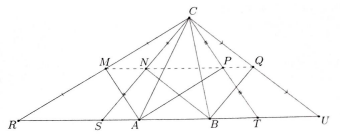
\includegraphics[scale=0.75]{img/img001.png}
    
    \item \iniTri. Seja $H$ seu ortocentro. Os pontos $L$ e $P$ são as projeções de $H$ sobre as bissetrizes interna e externa de $\angle ACB$, respectivamente. Prove que os pontos $M$, $L$ e $P$ são colineares, onde $M$ é o ponto médio de $AB$. \dica %Paralelogramos %Conjugados isogonais %Marque ângulos
    
    \item \iniTri. Uma reta passando por $C$ intersecta a bissetriz interna de $A$ e o circuncírculo de $\Delta ABC$ nos pontos $M$ e $N$, respectivamente. Uma circunferência $k_1$ passa por $A$ e toca $CM$ nos pontos $P$ e $Q$, respectivamente. Prove que os pontos $N$, $P$ e $Q$ são colineares. \dica %Marcação de ângulos
    
    \item Seja $\angle AOC$ um ângulo. O ponto $B$ fica sobre a semirreta $OA$ e o ponto $D$ fica sobre a semirreta $OC$. Além disso, $AB=CD$, $A$ fica entre $O$ e $B$, e $C$ fica sobre $O$ e $D$. Os circuncírculos de $\Delta ADO$ e $\Delta BOC$ intersectam-se novamente no ponto $K$. Prove que $OK$ é bissetriz interna de $\angle AOC$. \dica %Marque ângulos %Semelhança de triângulos %Definição de bissetriz
    
    \item Seja $ABC$ ($AC>BC$) um triângulo, seja $CL$ ($L\in AB$) sua bissetriz interna, e seja $O$ seu circuncentro. Denote os circuncentros de $\Delta ALC$ e $\Delta BLC$ por $O_1$ e $O_2$, respectivamente. Prove que $OO_1=OO_2$. \dica %Marcação de ângulos %Lei dos Senos %Lei dos Cossenos
    
    \item \iniTri. Seja $CL$ ($L\in AB$) uma bissetriz interna. O incírculo de $\Delta ALC$ toca $AC$, $AL$ e $CL$ nos pontos $M$, $N$ e $P$, respectivamente, e o $C$-exincírculo de $\Delta BCL$ toca as retas $BL$, $CB$ e $CL$ nos pontos $Q$, $R$ e $S$, respectivamente. Prove que cada uma das triplas de pontos $M$, $N$, $S$ e $P$, $Q$, $R$ são colineares. \dica %Trigonometria %Teorema do Bico %Teorema de Menelaus
    
    \item \iniTri. Sejam $AA^{\prime}$ e $BB^{\prime}$ alturas e $k$ o incírculo centrado em $I$. As retas $AI$ e $BI$ intersectam $BC$ e $AC$ nos pontos $F$ e $G$ respectivamente. A circunferência $k$ toca $BC$ e $CA$ nos pontos $D$ e $E$ respectivamente. Se $A^{\prime}B^{\prime}\cap GF=X$, prove que os pontos $E$, $D$ e $X$ são colineares. \dica %Razão anarmônica %Teorema de Tales %Teorema da bissetriz %Semelhança de triângulos
    
    \item \iniTri. Seja $CL$ bissetriz interna e $I$ incentro. A mediatriz do segmento $CL$ intersecta as bissetrizes internas de $\angle BAC$ e $\angle ABC$ nos pontos $M$ e $N$, respectivamente. Prove que o quadrilátero $MINC$ é cíclico. \dica %Marcação de ângulos
    
    \item \iniTri. Seja $I$ seu incentro. Os pontos $Y\in AI$ e $X\in BI$ são escolhidos de forma que $\angle XCA=\angle YCB$. Prove que as retas $AX$, $CI$ e $BY$ são concorrentes. \dica %Teorema de Desargues %Aplique razões em áreas %Teorema da bissetriz %Teorema de Ceva
    
    \item \iniTri. Sejam $AM$ e $BN$ bissetrizes internas que se intersectam em $I$. Pontos $L$ e $K$ são escolhidos sobre a reta $AB$ tais que $LN$ e $CN$ são simétricas com respeito a $BN$, e tais que $CM$ e $KM$ são simétricas com respeito a $AM$. Seja $D=LN\cap KM$. Prove que $DI\perp AB$. \dica %Marque ângulos %Exincentro %Deduza que $I$ é incentro de outro triângulo
    
    \item Seja $ABC$ ($AC>BC$) um triângulo de alturas $AA_1$ e $BB_1$, que se intersectam no ponto $H$. As bissetrizes internas de $\angle HAC$ e $\angle HBC$ se intersectam no ponto $L$. Sejam $M$ e $N$ os pontos médios de $AB$ e $CH$, respectivamente. Prove que os pontos $M$, $L$ e $N$ são colineares. \dica %Marque ângulos
    
    \item \iniTri. Seja $C_2$ o ponto médio de $AB$. As retas tangentes ao circuncírculo de $\Delta ABC$ em $A$ e $B$ se intersectam no ponto $N$. Prove que $\angle ACC_2=\angle BCN$. \dica %Aplique várias leis dos senos
    
    \item \iniTri. Os pontos $D$ e $E$ são escolhidos sobre os lados $AC$ e $BC$ de tal forma que o quadrilátero $ABED$ é cíclico. Seja $M$ o ponto médio de $AB$ e seja $F$ a interseção das retas tangentes ao circuncírculo de $\Delta DEC$ nos pontos $D$ e $E$. Prove que os pontos $M$, $F$ e $C$ são colineares. \dica %Conjugadas isogonais %Semelhança de triângulos %Marcação de ângulos
    
    \item \iniTri. Seja $k$ seu circuncírculo. As retas tangentes a $k$ por $A$ e $B$ se intersectam no ponto $D$. Digamos que $CD$ intersecte $k$ uma segunda vez no ponto $E$. As projeções de $E$ sobre $AB$, $BC$ e $CA$ são $N$, $P$ e $M$, respectivamente. Prove que $N$ é o ponto médio de $PM$. \dica %Reta de Simson %Lei dos senos
    
    \item \iniTri. As retas tangentes a seu circuncírculo pelos pontos $A$ e $B$ se intersectam em $T$. A reta $CT$ intersecta o circuncírculo de $\Delta ABC$ uma segunda vez no ponto $D$. Seja $CL$ ($L\in AB$) bissetriz interna de $\angle ACB$. Prove que $DL$ é bissetriz interna de $\angle ADB$. \dica %Simedianas %Ache um quadrilátero harmônico %Teorema da bissetriz interna
    
    \item \iniTri. As retas tangentes ao seu circuncírculo pelos pontos $A$ e $B$ se intersectam em $T$. A reta $CT$ intersecta o circuncírculo de $\Delta ABC$ uma segunda vez no ponto $D$. Seja $E$ a reflexão de $D$ com respeito a $AB$, e seja $M$ o ponto médio de $AB$. Prove que os pontos $C$, $E$ e $M$ são colineares. \dica %Conjugadas isogonais
    
    \item \iniTri. As retas tangentes a seu circuncírculo pelos pontos $A$ e $B$ se intersectam em $T$. A reta $CT$ intersecta o circuncírculo de $\Delta ABC$ uma segunda vez no ponto $D$. Seja $N\in CD$ um ponto tal que $\angle NBC=\angle ACN$. Prove que $\angle BCN=\angle CAN$. \dica %Simediana %Ache um quadrilátero harmônico %Conjugadas isogonais
    
    \item \iniTri. Sejam $E$, $F$ e $M$ pontos médios de $AC$, $BC$ e $EF$, respectivamente. O segmento $CD$ é uma altura de $\Delta ABC$. Prove que os circuncírculos de $\Delta ECF$, $\Delta BDF$ e $\Delta ADE$ concorrem num ponto da reta $DM$. \dica %Ponto fantasma %Marcação de ângulos %Congruência de triângulos
    
    \item \iniTri. Seja $M$ o ponto médio de $AB$ e seja $D$ o ponto de interseção das retas tangentes ao circuncírculo de $\Delta ABC$ pelos pontos $A$ e $B$. As projeções de $D$ sobre as retas $CA$ e $CB$ são $E$ e $F$, respectivamente. Prove que $CM\perp EF$. \dica %Ache um quadrilátero cíclico %Seja $H=CM\cap EF$ %Marcação de ângulos
    
    \item \iniTri. Seja $N$ o ponto médio da altura $CD$ e seja $M$ o ponto médio de $AB$. Seja $L$ o ponto de Lemoine de $\Delta ABC$. Prove que os pontos $N$, $L$ e $M$ são colineares. \dica %Propriedades do ponto de Lemoine %Teorema de Steiner
    
    \item Seja $k$ uma circunferência. Um ponto $C$ é escolhido exterior a $k$. As retas tangentes $k$ por $C$ tocam a circunferência nos pontos $A$ e $B$. Prove que o incentro de $\Delta ABC$ fica sobre $k$. \dica %Marcação de ângulos %Definição do incentro
    
    \item As circunferências $k_1$ e $k_2$ se tocam externamente no ponto $I$. Sejam $l_1$ e $l_2$ as retas tangentes externas comuns às duas circunferências. Os pontos de tangência de $l_1$ e $l_2$ a $k_2$ são $A$ e $B$, respectivamente. Os pontos de tangência de $l_1$ e $l_2$ a $k_1$ são $D$ e $C$, respectivamente. Prove que o quadrilátero $ABCD$ é inscritível. \dica %Use o problema anterior %Angle chasing
    
    \item \iniTri. $I$ é o incentro do triângulo. O incírculo de $\Delta ABC$ toca $AB$ em $N$. O $C$-exincírculo de $\Delta ABC$ toca $AB$ em $M$. Sejam $P$ e $Q$ as projeções ortogonais de $A$ e $B$ sobre a reta $CI$, respectivamente. Prove que os pontos $P$, $M$, $Q$ e $N$ ficam sobre uma circunferência de diâmetro $MN$. \dica %Ache um quadrilátero cíclico %Marque ângulos
    
    \item \iniTri. Seja $\omega$ seu incírculo, de centro $I$. Denote a projeção ortogonal de $B$ sobre $AI$ por $K$. Sejam $N$ e $M$ os pontos tangência de $AC$ e $BC$ por $\omega$, respectivamente. Prove que os pontos $M$, $N$ e $K$ são colineares. \dica %Marque ângulos para achar um quadrilátero cíclico %Prove a colinearidade por ângulos
    
    \item \iniTri. Seja $\omega$ seu incírculo, de centro $I$. Digamos que $AB$ toque $\omega$ em $N$. Sejam $K$ e $M$ os pontos médios de $CN$ e $AB$, respectivamente. Prove que $K$, $I$ e $M$ são colineares. \dica %Teorema de Newton %Note que um triângulo pode ser interpretado como um quadrilátero degenerado
    
    \item \iniTri. Seja $k$ seu incírculo, de centro $I$. Digamos que $AB$ toque $k$ no ponto $P$. Seja $CH$ ($H\in AB$) uma altura de $\Delta ABC$. Denote o ponto médio de $CH$ por $M$. Seja $k_C(I_C)$ o $C$-exincírculo de $\Delta ABC$, e digamos que ele toque $AB$ em $F$. Prove que os pontos $M$, $I$ e $F$ são colineares, e prove que os pontos $M$, $P$ e $I_C$ são colineares. \dica %Reflita $P$ com relação a $I$ %Ache uma boa homotetia %Aplique o Teorema de Steiner num trapézio da figura   
    
    \item \iniTri. Digamos que seu incírculo toque os lados $BC$, $CA$ e $AB$ nos pontos $F$, $E$ e $D$, respectivamente. Digamos também que seu $C$-exincírculo toque as retas $BC$, $CA$ e $AB$ nos pontos $Q$, $P$ e $M$, respectivamente. Seja $MN$ ($N\in PQ$) uma altura em $\Delta PMQ$, e seja $DH$ ($D\in EF$) uma altura em $\Delta EDF$. Prove que $\angle ACN=\angle BCH$. \dica %Trigonometria
    
    \item \iniTri. Sejam $\omega_X(I_X)$ seus $X$-exincírculos para $X\in\{A,B,C\}$. Digamos que $\omega_A$ toque $AB$, $AC$ e $BC$ em $P$, $Q$ e $E$, respectivamente, assim como $\omega_B$ toca $BC$, $BA$ e $CA$ em $N$, $M$ e $D$, respectivamente. Diremos ainda que $PE\cap MN=R$ e $MD\cap PQ=S$. Prove que os pontos $I_B$, $R$, $C$, $S$ e $I_A$ são colineares. \dica %Marcação de ângulo %Lei dos Senos
    
    \item \iniTri. Sejam $\omega_X(I_X)$ seus $X$-exincírculos para $X\in\{A,B,C\}$. Digamos que $\omega_A$ toque $AB$, $AC$ e $BC$ em $P$, $Q$ e $E$, respectivamente, assim como $\omega_B$ toca $BC$, $BA$ e $CA$ em $N$, $M$ e $D$, respectivamente. Seja $PE\cap MD=F$. Prove que $CF=r$, onde $r$ é o inrraio de $\Delta ABC$. \dica %Marque ângulos e aplique Lei dos Senos
    
    \item \iniTri. Sejam $\omega_X(I_X)$ seus $X$-exincírculos para $X\in\{A,B,C\}$. Digamos que $\omega_A$ toque $AB$, $AC$ e $BC$ em $P$, $Q$ e $E$, respectivamente, assim como $\omega_B$ toca $BC$, $BA$ e $CA$ em $N$, $M$ e $D$, respectivamente. Sejam $PE\cap MD=U$ e $PQ\cap MN=F$. Prove que $CF\perp AB$ e que $CU\perp AB$. \dica %Marque ângulos %Lei dos Senos %Observe $\Delta MPF$
    
    \item \iniTri. Sejam $\omega_X(I_X)$ seus $X$-exincírculos para $X\in\{A,B,C\}$. Digamos que $\omega_A$ toque $BC$ em $N$, assim como $\omega_B$ toca $CA$ em $M$ e $\omega_C$ toca $CA$ e $CB$ em $P$ e $Q$, respectivamente. Prove que as retas $PQ$, $MN$ e $AB$ concorrem. \dica %Teorema de Menelaus
    
    \item \iniTri. Seja $K$ o ponto médio de $AB$. A reta $CL$ ($L\in AB$) é a bissetriz interna de $\angle ACB$. O $B$-exincírculo de $\Delta ABC$ toca $AC$ no ponto $N$. O $A$-exincírculo de $\Delta ABC$ toca $BC$ no ponto $P$. Seja $M$ ponto médio de $NP$. Prove que $KM\parallel CL$. \dica %Marcação de ângulo %Base média %Teorema da Bissetriz
    
    \item \iniTri. Seja $\omega_A$ seu $A$-exincírculo, e $\omega_B$ seu $B$-exincírculo. $\omega_A$ toca $AB$ e $BC$ em $Q$ e $N$, respectivamente, assim como $\omega_B$ toca $AB$ e $AC$ em $P$ e $M$, respectivamente. Prove que as mediatrizes de $AN$ e $BM$, e a bissetriz interna de $\angle ACB$ são concorrentes. \dica %Ponto fantasma %Seja $L$ a interseção das duas mediatrizes %Triângulos congruentes
    
    \item \iniTri. Seja $k$ seu circuncírculo. Seja $M$ o ponto médio de $AB$, e seja $N$ o ponto médio do arco $ACB$. Sejam $I_1$ e $I_2$ os incentros de $\Delta ACM$ e $\Delta BCM$, respectivamente. Prove que os pontos $N$, $C$, $I_1$ e $I_2$ são concíclicos. \dica %Marcação de ângulo %Conjugadas isogonais
    
    \item \iniTri. Seja $CM$ uma mediana. Sejam $k_1(I_1)$ e $k_2(I_2)$ os incírculos de $\Delta ACM$ e $\Delta BCM$, respectivamente. Sejam $k_3(I_3)$ e $k_4(I_4)$ os $M$-exincírculos de $\Delta ACM$ e $\Delta BCM$, respectivamente. Prove que os pontos $I_1$, $I_2$, $I_3$ e $I_4$ são concíclicos. \dica %Angle chasing %Semelhança de triângulos %Use áreas para determinar razões entre segmentos %Potência de ponto
    
    \item \iniTri. Seja $k$ seu incírculo de centro $I$. Seja $k_1$ a circunferência que passa por $A$ e $B$, e que toca $k$ no ponto $T$. Seja $CH$ uma altura em $\Delta ABC$, e seja $M$ o ponto médio de $CH$. Seja $P$ o ponto de tangência de $AB$ com $k$. Prove que os pontos $P$, $M$ e $T$ são colineares. \dica %Eixo radical %Trigonometria %Semelhança de triângulos
    
    \item \iniTri. Sejam $AA_1$, $BB_1$ e $CC_1$ alturas. Sejam $C_2$, $A_2$ e $B_2$ os pontos de tangência do incírculo de $\Delta ABC$ com $AB$, $BC$ e $CA$, respectivamente. Denote os pontos médios de $AA_1$, $BB_1$ e $CC_1$ por $M$, $N$ e $P$, respectivamente. Prove que as retas $MA_2$, $NB_2$ e $PC_2$ são concorrentes. \dica %Eixo radical %Use o problema anterior
    
    \item \iniTri. Seja $\omega(I)$ seu incírculo, que toca $AB$ em $M$. Seja $L$ a reflexão de $M$ com respeito a $I$. Sejam $AI\cap BC=N$, $BI\cap AC=P$ e $PN\cap IC=K$. Seja $H$ a projeção de $C$ sobre $AB$. Prove que os pontos $L$, $K$ e $H$ são colineares. \dica %Teorema de Menelaus em $\Delta CSI$ %Teorema de Tales %Triângulos semelhantes
    
    \item \iniTri. Seja $\omega$ seu incírculo, que toca os lados $AB$, $BC$ e $CA$ nos pontos $M$, $N$ e $P$, respectivamente. Uma circunferência $k_1$ é construída de forma que toque $AB$ em $M$. Seja $L$ o ponto de interseção das retas tangentes a $k_1$ por $A$ e $B$ (distintas de $AB$). Digamos que $k_1$ toque $LA$ e $LB$ nos pontos $S$ e $Q$, respectivamente. Prove que os pontos $P$, $N$, $Q$ e $S$ são concíclicos. \dica %Marcação de ângulo
    
    \item \iniTri. Seja $\omega(I)$ seu incírculo, que toca $BC$ e $CA$ nos pontos $M$ e $N$, respectivamente. Seja $D$ a projeção de $A$ sobre $BI$, e seja $T$ a projeção de $I$ sobre $CD$. Sejam $P$ e $Q$ os pontos de interseção de $\omega$ com $BD$. Prove que os pontos $P$, $Q$, $C$ e $T$ são concíclicos. \dica %Observe o pentágono $IMCTN$ %Prove que $D$, $N$ e $M$ são colineares %Potência de ponto
    
    \item \iniTri. Seja $\omega$ seu incírculo, que toca $AB$ em $D$. Seja $CD\cap\omega=E\neq D$. A circunferência de centro $B$ e raio $BD$ intersecta $CD$ no ponto $F\neq D$. Seja $BF\cap AE=K$. Prove que $KF=FB$. \dica %Teorema de Menelaus %Trigonometria %Lei dos Senos %Truque da Cotangente
    
    \item \iniTri. Seja $\omega(I)$ seu incírculo, que toca os lados $AB$, $BC$ e $CA$ nos pontos $N$, $Q$ e $P$, respectivamente. Seja $NI\cap PQ=E$. Seja $F$ o ponto tal que $CF=CP$, $CF\parallel AB$, e $F$ e $A$ ficam em semiplanos distintos, com respeito a $BC$. Prove que os pontos $A$, $E$ e $F$ são colineares. \dica %Trigonometria %Truque da Cotangente
    
    \item \iniTri. Seja $\omega$ seu incírculo, que toca os lados $AB$, $BC$ e $CA$ nos pontos $M$, $F$ e $E$, respectivamente. Seja $CM\cap\omega = N\neq M$. Seja $l\parallel AB$ uma reta que passa por $C$. Os pontos $P$ e $Q$ são os pontos de interseção de $l$ com as retas $ME$ e $MF$, respectivamente. Prove que $\angle ENF=\angle PNQ$. \dica %Angle chasing %Ache quadriláteros cíclicos
    
    \item \iniTri. Seja $\omega$ seu incírculo, que toca os lados $BC$ e $CA$ nos pontos $D$ e $F$, respectivamente. Seja $AD\cap BF=G$. Denote o ponto médio de $FD$ por $M$. Sejam $K$ e $L$ as reflexões de $F$ e $D$ com respeito a $A$ e $B$, respectivamente. Prove que $MG\perp KL$. \dica %Trigonometria %Teorema de Menelaus %Lei dos Senos
    
    \item \iniTri. Digamos que $AC\geq BC$ e que $k$ seja seu incírculo, que toca os lados $BC$, $CA$ e $AB$ nos pontos $D$, $E$ e $F$, respectivamente. Sejam $L$ e $K$ as respectivas reflexões de $A$ e $B$ com respeito a $F$. As retas que passam por $L$ e $K$, perpendiculares a $AB$, intersectam $CB$ e $CA$ em $N$ e $M$, respectivamente. Prove que $MN$ toca $k$. \dica %Ponto fantasma %Retas polares e polos
    
    \item \iniTri. Seja $\omega$ seu incírculo, que toca os lados $AB$, $BC$ e $CA$ nos pontos $M$, $N$ e $P$, respectivamente. Seja $T$ a interseção do segmento $CI$ com $\omega$. Seja $MP\cap AT=R$ e $MN\cap BT=Q$. Prove que $RQ\perp IC$. \dica %Prove que $PN\parallel RQ$ %Use trigonometria e áreas %Teorema de Ceva
    
    \item Seja $ABC$ um triângulo isósceles ($AC=BC$) e digamos que $AC>AB$. Seu incírculo $\omega$ toca $AB$ e $CA$ em $M$ e $N$, respectivamente. Seja $P$ um ponto no lado $BC$ tal que $AP=AB$. Seja $I_1$ o incentro de $\Delta APC$. As retas $AI_1$ e $MN$ se intersectam em $K$. Prove que $K$ é o ponto médio de $AI_1$. \dica %Angle chasing
    
    \item \iniTri. Seja $I$ seu incentro. Seja $k_2(I_2)$ uma circunferência que toca os segmentos $AC$ e $BC$. Seja $k_1(I_1)$ uma circunferência que toca $AB$ em $G$, $AC$, e $k_2$ em $D$. Seja $k_3(I_3)$ uma circunferência que toca $AB$ em $T$, $BC$, e $k_2$ em $F$. Prove que $I$ fica sobre a mediatriz do segmento cujas extremidades são os pontos de interseção dos segmentos $AI$ e $BI$ com o circuncírculo de $\Delta GTF$. \dica %Prove que $GTFD$ é cíclico %Lei dos Senos %Triângulos congruentes
    
    \item 4.5.29
    
    \item Sejam $m_A$, $m_B$ e $m_C$ círculos de Malfatti de um triângulo $ABC$ de incentro $I$. Sejam $m_A\cap m_B=T_C$, $m_B\cap m_C=T_A$ e $m_A\cap m_C=T_B$. As circunferências $m_A$ e $m_B$ tocam $AB$ em $X$ e $Y$, respectivamente. Prove que o quadrilátero $XYT_AT_B$ é inscrito numa circunferência, e digamos que essa circunferência intersecte $AI$ e $BI$ nos pontos $M$ e $N$, respectivamente. Prove também que $AM=AX$ e $BN=BY$. \dica %Centro radical e eixos radicais
    
    \item 4.5.31
    
    \item \iniTri. Sejam $D$ e $E$ pontos sobre $AB$ ($D$ fica entre $A$ e $E$). Sejam $k_1$, $k_2$, $k_3$ e $k_4$ os incírculos de $\Delta ADC$, $\Delta AEC$, $\Delta BDC$ e $\Delta BEC$, respectivamente. Prove que $AB$ e as retas tangentes externas (diferentes de $AB$) dos pares de círculos $(k_1,k_4)$ e $(k_2,k_3)$ são concorrentes.
    
    \item \iniTri. Seja $D$ um ponto arbitrário do segmento $AB$. Sejam $k_1$ e $k_2$ os incírculos de $\Delta ADC$ e $\Delta BDC$, respectivamente. Digamos que a reta tangente externa comum a $k_1$ e $k_2$ (distinta de $AB$) intersecta $CD$ em $K$. Prove que $CK=\frac{AC+BC-AB}{2}$. \dica %Lei do Bico
    
    \item \iniTri. Seja $k$ seu incírculo, que toca $AB$ em $E$. Seja $D$ um ponto sobre o segmento $AB$. Sejam $k_1(I_1)$ e $k_2(I_2)$ os incírculos de $\Delta ADC$ e $\Delta BDC$, respectivamente. Prove que $\angle I_1E_2=90^{\circ}$. \dica %Trigonometria %Truque da cotangente
    
    \item \iniTri. Seja $CH$ uma altura e digamos que seu incírculo toque $AB$ em $M$. Denote os incentros de $\Delta AHC$ e $\Delta BHC$ por $I_1$ e $I_2$, respectivamente. Um ponto $D_1$ é escolhido tal que $MI_2D_1I_1$ é um retângulo. Prove que este retângulo é um quadrado, e prove que $D_1$ fica sobre $CH$. \dica %Use o problema anterior %Seja $D\in CH$ tal que $\angle MI_1D=90^{circ}$ %Angle chasing %Ponto fantasma
    
    \item \iniTri. Seja $k$ seu circuncírculo. Seja $l$ a reta tal que $l\parallel AB$ e tal que $l$ intersecta $AC$ e $BC$ nos pontos $D$ e $E$, respectivamente. Digamos que $DE$ intersecte $k$ nos pontos $P$ e $Q$, respectivamente ($D$ fica entre $P$ e $E$). Seja $k_1$ a circunferência que toca os segmentos $PD$, $DC$, e o arco menor $PC$ de $k$. Seja $k_2$ a circunferência que toca os segmentos $EQ$, $EC$, e o arco menor $QC$ de $k$. Digamos que $k_1$ toque $DC$ em $M$. Digamos que $k_2$ toque $EC$ em $N$. Prove que $MN\parallel l$. \dica %Lema de Sawayama %Angle chasing
    
    \item \iniTri. Seja $k$ seu circuncírculo. Os pontos médios dos arcos menores $BC$ e $AC$ são $M$ e $N$, respectivamente. As retas $AM$ e $BN$ se intersectam em $I$. Seja $k_1(N)$ a circunferência que toca $AC$, e seja $k_2(M)$ a circunferência que toca $BC$. Prove que uma das retas tangentes externas comuns a $k_1$ e $k_2$ passa por $C$, e a outra passa por $I$. \dica %Angle chasing %Teorema do trílio %Triângulos congruentes
    
    \item \iniTri. Seja $l$ uma reta que passa por $A$, que não intersecta o segmento $BC$. Sejam $k_1(O_1)$, $k_2(O_2)$ e $k_3(O_3)$ circunferências que tocam as retas $AB$, $BC$, $CA$ e $l$ ($k_1$ não toca $AC$, $k_2$ não toca $BA$ e $k_3$ não toca $l$). Prove que o quadrilátero $O_1O_3O_2A$ é cíclico. \dica %Marcação de ângulo
    
    \item Usando a construção do problema anterior, prove que o ortocentro de $\Delta O_1O_2O_3$ fica sobre $BC$. \dica %Pense em reflexões com respeito a $\Delta O_1O_2O_3$
    
    \item Seja $ABCD$ um quadrilátero convexo. Os quatro exincírculos do quadrilátero são construídos. Sejam $O_1$ e $O_2$ os centros das circunferências que tocam os segmentos $AD$ e $BC$. As outras duas circunferências tocam os segmentos $AB$ e $DC$ em $L$ e $K$, respectivamente. Seja $M$ o ponto médio de $O_1O_2$. Prove que $MK=ML$. \dica %Complete as retas tangentes %Teorema do Bico %Teorema de Pitágoras
    
    \item \iniTri. Sejam $AF$, $BD$ e $CE$ alturas. Digamos que seu incírculo toque $AB$ e $AC$ nos pontos $K$ e $L$, respectivamente. Sejam $I_1$ e $I_2$ os incentros de $\Delta AED$ e de $\Delta CDF$, respectivamente. Prove que $KI_1=LI_1=LI_2$. \dica %Busque triângulos semelhantes %Roto-homotetia
    
    \item \iniTri. Sejam $CC_1$ e $CC_2$, $AA_1$ e $AA_2$, $BB_1$ e $BB_2$ três pares de segmentos isogonalmente conjugados com respeito a $\Delta ABC$. Temos que $C_1\in AB$, $C_2\in AB$, $B_1\in AC$, $B_2\in AC$, $A_1\in BC$, e $A_2\in BC$. Sejam $AA_1\cap CC_2=X$, $BB_1\cap AA_2=Y$, e $CC_1\cap BB_2=Z$. Prove que se os quadriláteros $AC_1ZB_2$ e $BA_1XC_2$ são circunscritíveis, então o quadrilátero $B_1YA_2C$ também é circunscritível. \dica %Trigonometria %Teorema de Ceva
    
    \item Seja $ABCD$ um quadrilátero circunscritível e incírculo $k$. Digamos que as semirretas $DA$ e $CB$ se intersectem em $E$, e digamos que as semirretas $DC$ e $AB$ se intersectem em $F$. Seja $H$ a projeção de $B$ sobre a reta $EF$. Sejam $k_1$ e $k_2$ os incírculos de $\Delta ABE$ e $\Delta BCF$, respectivamente. Sejam $I_1$ e $I_2$ seus respectivos centros. Sejam $HP$ e $HQ$ as retas tangentes de $H$ respectivamente a $k_1$ e $k_2$ ($P\in k_1$ e $Q\in k_2$). Prove que $\angle I_1HP=\angle I_2HQ$. \dica %Teorema de Monge %Roto-homotetia
    
    \item Prove o Lema do Incentro-Exincentro, isto é, para um triângulo $ABC$ de incentro $I$ e circuncírculo $k$, se $M$ é o segundo ponto de interseção de $CI$ com $k$, então $MA=MB=MI$. \dica %Marcação de ângulos
    
    \item \iniTri. Seja $I$ seu incentro. Seja $M$ o ponto médio de $AB$, e seja $L$ o ponto médio do arco $ACB$. Prove que $\angle ILC=\angle IMB$. \dica %Exincentros %Marcação de ângulos %Alternativamente, você pode usar muita trigonometria, com truque da cotangente
    
    \item Prove a fórmula de Euler, isto é, que para um triângulo $ABC$, $OI^2=R^2-2Rr$, onde $O$ e $I$ são o circuncentro e incentro, respectivamente, e $R$ e $r$ são o circunraio e o inraio, respectivamente. \dica %Marque ângulos %Semelhança de triângulos %Lema do incentro-exincentro %Potência de ponto
    
    \item \iniTri. Seja $k$ seu circuncírculo, $\omega$ seu incírculo, e $I$ seu incentro. A reta que passa por $I$ e que é perpendicular a $CI$, intersecta a reta $AB$ em $M$. Seja $K$ a segunda interseção de $k$ com $MC$. Prove que $IK\perp MC$. \dica %Angle chasing %Semelhança de triângulos %Potência de ponto
    
    \item \iniTri. Seja $\omega$ seu incírculo e $k$ seu circuncírculo. A circunferência $\omega$ toca $AB$, $BC$ e $CA$ nos pontos $M$, $N$ e $P$, respectivamente. Os pontos $R$, $S$ e $T$ são os pontos médios dos arcos menores $AB$, $BC$ e $CA$, respectivamente. Prove que as retas $MR$, $SN$ e $PT$ são concorrentes. \dica %Construa retas tangentes a $k$ %Homotetia
    
    \item \iniTri. Seja $\omega$ seu incírculo e $k$ seu circuncírculo. A circunferência $\omega$ toca $BC$, $CA$ e $AB$ nos pontos $D$, $E$ e $F$, respectivamente. Digamos que $ED\cap AB=K$. Prove que o ponto médio $M$ de $KF$ fica sobre o eixo radical de $k$ e $\omega$. \dica %Potência de ponto %Teorema de Menelaus
    
    \item Prove o Lema de Verrièr, isto é, dado um triângulo $ABC$, com circuncírculo $k$, e com incírculo $C$-mixtilinear $\omega$, que toca $AC$, $BC$ e $k$ nos pontos $E$, $F$ e $D$, respectivamente, prove que o incentro de $\Delta ABC$ é o ponto médio do segmento $EF$. \dica %Construa $DF\cap k$ e $DE\cap k$ %Prove que esses novos pontos são pontos médios de arcos %Teorema de Pascal %Teorema do Bico
    
    \item \iniTri. Seja $k$ seu circuncírculo. Seja $\omega$ seu incírculo $C$-mixtilinear, que toca $AC$, $BC$ e $k$ nos pontos $E$, $F$ e $X$, respectivamente. O ponto $D$ é o ponto médio do arco $ACB$. Prove que os pontos $X$, $D$ e o ponto médio de $EF$ são colineares. \dica %Use o problema anterior %Ponto fantasma %Angle chasing
    
    \item \iniTri. Seja $k$ seu circuncírculo. Seja $\omega$ seu incírculo $A$-mixtilinear, que toca $AC$, $AB$ e $k$ nos pontos $E$, $F$ e $X$, respectivamente. Os pontos $P$ e $Q$ são os pontos médios dos arcos menores $AC$ e $AB$, respectivamente. Os pontos $M$ e $N$ são os pontos médios de $AE$ e $AF$, respectivamente. Prove que os pontos $P$, $M$, $N$ e $Q$ são colineares. \dica %Marque ângulos %Prove que $P$, $E$ e $X$ são colineares, assim como $Q$, $F$ e $X$ são colineares %Semelhança de Triângulos %Potência de pontos %Eixo radical
    
    \item \iniTri. Seja $k$ seu circuncírculo. Seja $M$ o ponto médio do arco menor $AB$ de $k$. Seja $G$ o ponto diametralmente oposto a $C$ com respeito a $k$, e seja $AG\cap CM=X$. Seja $k_1$ o incírculo $C$-mixtilinear de $\Delta ABC$. O segmento $GH$ ($H\in k_1$) é tangente a $k_1$. Prove que $GH=GX$. \dica %Eixo radical %Trigonometria %Lema de Verrièr %Lei dos senos
    
    \item \iniTri. Seja $k$ seu circuncírculo. O incírculo $C$-mixtilinear $k_1$ toca $k$ no ponto $M$, e as retas $AC$ e $BC$ nos pontos $F$ e $L$, respectivamente. Seja $FL\cap CM=N$. Prove que $\angle ANF=\angle BNL$. \dica %Marcação de ângulos %Semelhança de triângulos %Teorema de Casey %Trigonometria
    
    \item \iniTri. Seja $k$ seu circuncírculo. Seja $D$ um ponto arbitrário no arco menor $AB$ de $k$. A circunferência $k_1$ toca $k$ internamente no ponto $D$ e a reta $BC$ no ponto $P$. A circunferência $k_2$ toca $k$ internamente no ponto $D$ e a reta $AC$ no ponto $H$. O ponto $I$ é o incentro de $\Delta ABC$. Prove que os pontos $H$, $I$ e $P$ são colineares. \dica %Prove que $DH\cap k=L$ é ponto médio do arco menor $AC$, assim como $DP\cap k=M$ com o arco menor $BC$ %Teorema de Pascal
    
    \item \iniTri. Seja $k$ seu circuncírculo e $k_1$ seu incírculo $C$-mixtilinear. Seu incírculo $k_2$ toca $AB$ no ponto $Q$. Prove que $\angle APQ=\angle BAC$ e $\angle BPQ=\angle ABC$. \dica %Trigonometria com lei dos senos %Cotangentes
    
    \item \iniTri. Seja $I$ seu incentro. Seja $k$ um círculo arbitrário que passe por $A$ e $B$. O círculo $k_1$ toca $AC$ e $BC$ nos pontos $N$ e $M$, respectivamente. Ele também toca o arco menor $AB$ de $k$ internamente no ponto $X$. Prove que $\angle AXI=\angle IXB$. \dica %Teorema de Casey %Marcação de ângulos %Lei dos Senos
    
    \item \iniTri. Seja $k$ seu circuncírculo. O círculo $C$-mixtilinear $k_1$ toca $k$ no ponto $P$. Seja $Q$ um ponto arbitrário no arco $AB$ de $k$ que não contém $C$. Os pontos $I_1$ e $I_2$ são os incentros de $\Delta AQC$ e $\Delta QBC$, respectivamente. Prove que o quadrilátero $QPI_2I_1$ é cíclico. \dica %Sejam $M$ e $N$ os pontos médios dos arcos $BC$ e $AC$ de $k$ %Seja $X$ a interseção das tangentes a $k$ por $C$ e por $P$ %Marque ângulos procurando colinearidades %Centro radical
    
    \item \iniTri. Seja $k$ seu circuncírculo, $\omega$ seu incírculo. O incírculo $C$-mixtilinear $k_1$ toca $k$ no ponto $K$. O ponto $M$ no arco $AKB$ é arbitrário. As retas tangentes por $M$ a $\omega$ intersectam $AB$ nos pontos $E$ e $F$. Prove que o quadrilátero $MEFK$ é cíclico. \dica %Ponto fantasma %Marcação de ângulo e triângulos semelhantes %Teorema da bissetriz
    
    \item \iniTri. Seja $k$ seu circuncírculo. Seu $C$-exincírculo $k_1$ toca $AB$ no ponto $F$. Seu incírculo $C$-mixtilinear $k_2$ toca $k$ no ponto $D$. Prove que $\angle ACF=\angle BCD$. \dica %Inversão com um bom raio %Composição de inversão e reflexão
    
    \item \iniTri. Seja $k$ seu circuncírculo. Seu incírculo $k_1$ toca o segmento $AB$ no ponto $F$. Seu exincírculo $C$-mixtilinear $k_2$ toca $k$ no ponto $D$. Prove que $\angle ACF=\angle BCD$. \dica %Use o problema anterior
    
    \item Prove o Lema de Sawayama: \iniTri. Seja $k$ seu circuncírculo. Seja $D$ um ponto arbitrário em $AB$. A circunferência $k_1$ toca os segmentos $AD$ e $CD$, assim como $k$ internamente num ponto do arco $AC$. Digamos que $k_1$ toque $AB$ em $F$, e $CD$ em $M$. O ponto $I$ é o incentro de $\Delta ABC$. Prove que os pontos $F$, $M$ e $I$ são colineares. \dica %Teorema de Casey %Teorema da Bissetriz %Teorema de Menelaus
    
    \item \iniTri. Seja $k$ seu circuncírculo. O ponto $D$ fica sobre o segmento $AB$. A circunferência $k_1$ toca $AB$ no ponto $F$, toca $CD$ no ponto $M$ e toca $k$ internamente no ponto $K$, sobre o arco menor $AC$. O ponto $I$ é o incentro de $\Delta ABC$, e o ponto $I_1$ é o incentro de $\Delta ADC$. Prove que o pentágono $KI_1IMC$ é cíclico. \dica %Seja $L=CI\cap k$ %Angle chasing %Semelhança de triângulos %Potência de ponto
    
    \item Prove o Teorema de Thébault: \iniTri. Seja $k$ seu circuncírculo. O ponto $D$ fica sobre o segmento $AB$. A circunferência $k_1$ toca o segmento $AD$ no ponto $K$, o segmento $CD$ no ponto $E$, e a circunferência $k$ internamente num ponto do arco $AC$. A circunferência $k_2$ toca o segmento $BD$ no ponto $M$, o segmento $CD$ no ponto $N$, e a circunferência $k$ internamente num ponto do arco $BC$. O ponto $I$ é o incentro de $\Delta ABC$ e os pontos $I_1$ e $I_2$ são os centros de $k_1$ e $k_2$, respectivamente. Prove que os pontos $I$, $I_1$ e $I_2$ são colineares. \dica %Lema de Sawayama %Perpendicularidade e marcação de ângulo %Semelhança de triângulo
    
    \item \iniTri. Seja $k$ seu circuncírculo. O ponto $D$ fica sobre o segmento $AB$. A circunferência $k_1$ toca a circunferência $k$ internamente num ponto do arco $AC$, toca o segmento $AD$ no ponto $X$, e toca o segmento $CD$ no ponto $F$. A circunferência $k_2$ toca a circunferência $k$ internamente num ponto do arco $BC$, toca o segmento $BD$ em $G$, e toca o segmento $CD$ no ponto $K$. O ponto $I$ é o incentro de $\Delta ABC$. O segmento $YZ$ é a segunda reta tangente externa comum entre $k_1$ e $k_2$, tal que $Y\in k_1$ e $Z\in k_2$. Seja $ZK\cap FY=L$. Prove que os pontos $A$, $B$, $I$ e $L$ são concíclicos. \dica %Angle Chasing %Lema de Sawayama %Teorema de Thébault %Semelhança de Triângulos %Eixo e centro radical
    
    \item Seja $ABCD$ um quadrilátero cíclico de circuncírculo $k$. A circunferência $k_1$ toca a circunferência $k$ internamente num ponto do arco menor $AD$, toca o segmento $AC$ no ponto $F$, e toca o segmento $BD$ no ponto $E$. A circunferência $k_2$ toca a circunferência $k$ internamente num ponto do arco menor $BC$, toca o segmento $AC$ num ponto $N$, e toca o segmento $BD$ no ponto $K$. Os pontos $P$ e $Q$ são os pontos médios de $EK$ e $NF$, respectivamente. Os pontos $T$ e $S$ são os pontos médios dos arcos menores $CD$ e $AB$, respectivamente. Prove que os pontos $T$, $P$, $Q$ e $M$ são colineares. \dica %Eixo radical %Teorema de Casey
    
    \item Seja $CYBED$ um pentágono cíclico de circuncírculo $k$. A circunferência $k_1$ toca a reta $CB$ no ponto $N$, toca a reta $EY$, e toca a circunferência $k$ internamente num ponto do arco menor $CE$. A circunferência $k_2$ toca a reta $CB$ no ponto $M$, toca a reta $DY$, e toca a circunferência $k$ internamente num ponto do arco menor $BD$. A circunferência $k_3$ toca as retas $CD$ e $BE$, e a circunferência $k$ internamente no ponto $X$ do arco menor $CB$. Prove que o quadrilátero $XYNM$ é cíclico. \dica %Seja $A=CD\cap BE$ %Sejam $I$, $I_1$ e $I_2$ incentros de $\Delta CBA$, $\Delta CBD$ e $\Delta CBE$. Prove que $CXI_2I$ e $BXI_1I$ são cíclicos %Lema de Sawayama %Marcação de ângulo %Potência de ponto
    
    \item Seja $ABCD$ um quadrilátero cíclico de circuncírculo $k$. A circunferência $k_1$ toca as retas $AC$ e $BD$, e a circunferência $k$ internamente no ponto $E$ sobre o arco menor $AD$. A circunferência $k_2$ toca as retas $AC$ e $BD$, e a circunferência $k$ internamente no ponto $Z$ sobre o arco menor $BC$. Sejam $X\in k_2$ e $K\in k_1$ pontos tais que $XK$ é uma reta tangente externa comum a $k_1$ e $k_2$, com $C$ e $X$ sobre o mesmo semi-plano com respeito a $EZ$. A circunferência $k_3$ toca $k_1$ e $k_2$ externamente. Seja $k_3\cap BD=M$, tal que $M$ é o ponto de interseção mais próximo de $D$, e seja $k_3\cap AC=T$, tal que $T$ é o ponto de interseção mais próximo de $C$. Prove que $MT\parallel XK\parallel CD$. \dica %Eixo radical %Homotetia %Potência de ponto
    
    \item (Círculo de Euler) \iniTri. Seja $H$ seu ortocentro. Prove que os pontos médios de seus lados, os pés de suas alturas, e os pontos médios dos segmentos $AH$, $BH$ e $CH$ são concíclicos. \dica %Angle chasing %Atente-se a quadriláteros cíclicos
    
    \item \iniTri. Sejam $k$, $k_A$, $k_B$ e $k_C$ o incírculo e os três exincírculos, respectivamente. Sejam $A_1$, $B_1$ e $C_1$ os pontos médios de $BC$, $CA$ e $AB$, respectivamente. Prove que o circuncírculo $\omega$ de $\Delta A_1B_1C_1$ é tangente a todas as outras circunferências. \dica %Inversão com bom raio %Angle chasing e semelhança de triângulos
    
    \item \iniTri. Seja $I$ seu incentro e $O$ seu circuncentro. Seja $P$ um ponto arbitrário na reta $OI$. Denote os pés das perpendiculares de $P$ a $AB$, $BC$ e $CA$ por $C_2$, $A_2$ e $B_2$, respectivamente. Prove que o ponto de Feuerbach $F$ fica sobre o circuncírculo de $\Delta A_2B_2C_2$. \dica %Teoremas de Fontene %Círculo de Euler %Teorema de Feuerbach (problema anterior)
    
    \item \iniTri. Sejam $AA_1$, $BB_1$ e $CC_1$ bissetrizes internas. Seja $F$ o ponto de Feuerbach de $\Delta ABC$. Prove que o quadrilátero $A_1B_1C_1F$ é cíclico. \dica %Teorema de Monge %Círculo de Euler %Fórmula de Euler %Teorema de Casey
    
    \item \iniTri. Seja $I$ seu incentro. Seu incírculo toca $AB$, $BC$ e $AC$ em $C_2$, $A_2$ e $B_2$, respectivamente. Os pontos médios de $AB$, $BC$ e $CA$ são $C_1$, $A_1$ e $B_1$, respectivamente. Seja $A_1B_1\cap A_2B_2=D$. Prove que o ponto de Feuerbach $F$ fica sobre a reta $DC_2$. \dica %Use os problemas anteriores %Teoremas de Fontene
    
    \item 4.8.6
    
    \item \iniTri. Denote os pontos médios de $AB$, $BC$ e $CA$ por $C_1$, $A_1$ e $B_1$, respectivamente. Denote os pontos de tangência dos exincírculos com os segmentos $AB$, $BC$ e $CA$ por $C_2$, $A_2$ e $B_2$, respectivamente. Seja $A_1B_1\cap A_2B_2=G$. Prove que o ponto de Feuerbach $F$ fica sobre a reta $GC_2$. \dica %Ponto de Bevan %Use os problemas anteriores %Teoremas de Fontene 
    
    \item \iniTri. Sejam $M$ e $N$ os pontos médios de $AB$ e $BC$, respectivamente. Denote o incírculo, o círculo de Euler e os exincírculos de $\Delta ABC$ por $k$, $k_1$, $k_A$, $k_B$ e $k_C$, respectivamente. Sejam $k\cap k_1=D$, $k_A\cap k_1=E$, $k_B\cap k_1=F$ e $k_C\cap k_1=G$. Prove que as retas $MN$, $DF$ e $EG$ são concorrentes. \dica %Inversão sobre a circunferência de diâmetro $KH$ %Trigonometria e contas %Eixo radical
    
    \item \iniTri. Seja $k$ seu circuncírculo. Seja $X$ um ponto arbitrário interno a $\Delta ABC$. Denote $AX\cap BC=A_1$, $BX\cap AC=B_1$ e $CX\cap AB=C_1$. A circunferência $k_A$ é externa a $\Delta ABC$, toca $k$ internamente, e também toca o segmento $BC$ no ponto $A_1$. As circunferências $k_B$ e $k_C$ são definidas analogamente. Denote o incírculo de $\Delta ABC$ por $\omega$. Prove que existe uma circunferência que é tangente externamente a $k_A$, $k_B$ e $k_C$, e internamente a $\omega$. \dica %Teorema de Casey
    
    \item (Círculo de Conway) \iniTri. Os pontos $P$ e $S$ ficam sobre a reta $AB$, tais que os pontos $P$, $A$, $B$ e $S$ estão nessa ordem, $AP=BC$ e $BS=AC$. Os pontos $R$ e $N$ ficam sobre a reta $BC$, tais que os pontos $R$, $B$, $C$ e $N$ estão nessa ordem, $CN=AB$ e $BR=AC$. Os pontos $M$ e $Q$ ficam sobre a reta $CA$, tais que os pontos $Q$, $A$, $C$ e $M$ estão nessa ordem, $CM=AB$ e $AQ=BC$. Prove que o hexágono $MNPQRS$ é cíclico. \dica %Comece por quadriláteros %Potência de ponto e eixo radical
    
    \item \iniTri. Os pontos $D$, $E$ e $F$ são os pontos médios dos lados $BC$, $CA$ e $AB$, respectivamente. O ponto $G$ é o baricentro de $\Delta ABC$. Prove que os circuncentros de $\Delta AFG$, $\Delta AEG$, $\Delta GDB$, $\Delta FGB$, $\Delta GDC$ e $\Delta EGC$ são concíclicos. \dica %Comece por quadriláteros %Eixos radicais
    
    \item As circunferências $k_1$, $k_2$ e $k_3$ são escolhidas de forma que $k_1\cap k_2=\{R,S\}$, $k_2\cap k_3=\{P,Q\}$ e $k_3\cap k_1=\{M,N\}$. Denote o centro radical de $k_1$, $k_2$ e $k_3$ por $X$. Os pontos $A$, $B$ e $C$ são escolhidos nas semirretas $XM$, $XQ$ e $XS$ após $M$, $Q$ e $P$, respectivamente. Sejam $AB\cap k_3=\{G,H\}$, $BC\cap k_2=\{I,J\}$ e $CA\cap k_1=\{K,L\}$. Prove que os pontos $H$, $I$, $J$, $K$, $L$ e $G$ são concíclicos. \dica %Eixo Radical %Quadrilátero cíclico
    
    \item \iniTri. Uma circunferência $k$ que passa por $A$ e $B$ intersecta os lados $AC$ e $BC$ nos pontos $E$ e $D$, respectivamente. Seja $AD\cap BE=G$. Denote os pontos médios de $AB$ e $DE$ por $M$ e $N$, respectivamente. Prove que a reta $CG$ é tangente ao circuncírculo de $\Delta MGN$. \dica %Denote as reflexões de $G$ com respeito a $M$ e $N$ por $K$ e $L$, respectivamente %Angle chasing %Triângulos semelhantes %Potência de ponto %Homotetia
    
    \item \iniTri. Os pontos $N$ e $M$ são escolhidos sobre os lados $AC$ e $BC$, respectivamente, de tal forma que $ABMN$ é cíclico. Sejam $AM\cap BN=D$ e $CD\cap AB=P$. Denote o ponto médio do segmento $AB$ por $Q$. Prove que o quadrilátero $MNQP$ é cíclico. \dica %Teorema de Menelaus %Teorema de Ceva %Potência de ponto
    
    \item \iniTri. Seja $k$ seu circuncírculo. Sejam $M$, $N$ e $P$ os pontos médios de $AB$, $BC$ e $CA$, respectivamente. Seja $D\in AB$ um ponto tal que $CD$ é tangente a $k$. Denote o circuncírculo de $\Delta MNP$ por $k_1$. Prove que o ponto $C$ fica sobre a reta polar de $D$ com respeito a $k_1$. \dica %Teorema de La Hire %Homotetia
    
    \item \iniTri. Seja $O$ seu circuncentro. Seja $k$ uma circunferência que passa por $C$ e $O$. Denote $k\cap AC=\{C,D\}$ e $k\cap BC=\{C,E\}$. Prove que o ortocentro de $\Delta DOE$ fica sobre $AB$. \dica %Marque ângulos
    
    \item \iniTri. Seja $k$ seu circuncírculo. O ponto $D$ é o ponto médio do arco $ACB$. Um ponto arbitrário $M$ é escolhido sobre o lado $AC$. O ponto $N\in BC$ satisfaz $AM=BN$. Prove que os pontos $C$, $D$, $N$ e $M$ são concíclicos. \dica %Marcação de ângulos %Semelhança de triângulos
    
    \item \iniTri. Seja $X$ um ponto arbitrário sobre $AB$. Os pontos $E$ e $F$ ficam sobre os lados $AC$ e $BC$ e são escolhidos de forma que os quadriláteros $AXFC$ e $BCEX$ são cíclicos. Seja $O$ o circuncentro de $\Delta EFC$. Prove que $OX\perp AB$. \dica %Angle chasing %Quadrilátero cíclico
    
    \item \iniTri. Seja $k$ seu circuncírculo. Sejam $M$ e $N$ pontos arbitrários sobre o lado $AB$, tais que $M$ fica entre $A$ e $N$. Os pontos $K\in AC$ e $L\in BC$ são escolhidos tais que $MK\parallel BC$ e $NL\parallel AC$. A reta $LK$ intersecta $k$ nos pontos $P$ e $Q$. Prove que o quadrilátero $MNQP$ é cíclico. \dica %Teorema de Menelaus %Potência de ponto
    
    \item Seja $ACBD$ um quadrilátero convexo tal que $AC=AD$ e $BC=BD$. O circuncírculo de $\Delta ABC$ intersecta $AD$ e $BD$ nos pontos $E$ e $F$, respectivamente. Prove que $\angle ECD=\angle FCD$. \dica %Angle chasing
    
    \item \iniTri. Seu incírculo é $\omega$ e seu incentro é $I$. Digamos que $\omega$ toque $AB$, $BC$ e $CA$ nos pontos $M$, $N$ e $P$, respectivamente. Seja $AB\cap PN=K$. Prove que $CM\perp KI$. \dica %Polo e reta polar %Teorema de La Hire
    
    \item \iniTri. Seu incírculo é $\omega$ e seu incentro é $I$. Digamos que $\omega$ toque $AB$, $BC$ e $CA$ nos pontos $M$, $N$ e $P$, respectivamente. Sejam $AB\cap PN=K$ e $CM\cap KN=L$. Prove que $IL\perp KC$. \dica %Use o problema anterior
    
    \item \iniTri. Seja $X$ um ponto interno ao triângulo. Os pontos $M$, $N$ e $P$ são os pés das perpendiculares de $X$ até $AB$, $BC$ e $CA$, respectivamente. Seja $Q$ o segundo ponto de interseção do circuncírculo de $\Delta MNP$ com $AB$, e digamos que as retas $AB$ e $PN$ se intersectem em $T$. Prove que $TX\perp CQ$. \dica %Teorema dos Eixos Radicais
    
    \item (Teorema de Brocard) Um quadrilátero não-trapézio $ABCD$ é inscrito numa circunferência de centro $O$. Seja $AC\cap BD=H$, $AB\cap CD=E$ e $AD\cap BC=F$. Prove que $FH\perp OE$. \dica %Polo e reta polar
    
    \item (Teorema de Brocard) Um quadrilátero não-trapézio $ABCD$ é inscrito numa circunferência de centro $O$. Seja $AC\cap BD=H$, $AB\cap CD=E$ e $AD\cap BC=F$. Prove que $OH\perp FE$. \dica %Use o problema anterior
    
    \item \iniTri. Seja $X$ um ponto arbitrário sobre $AB$. Denote os circuncírculos de $\Delta AXC$ e $\Delta BXC$ por $k_1$ e $k_2$, respectivamente. Os pontos $E\in AC$ e $F\in BC$ são escolhidos tais que $EX\parallel BC$ e $FX\parallel AC$. O ponto $M\in k_1$ é escolhido tal que $ME\perp AC$, e tal que $M$ e $X$ fiquem em semi-planos distintos com respeito a $AC$. O ponto $N\in k_2$ é escolhido tal que $NF\perp BC$, e tal que $N$ e $X$ fiquem em semi-planos distintos com respeito a $BC$. Prove que $\angle MXN=90^{\circ}$. \dica %Angle chasing %Triângulos semelhantes
    
    \item \iniTri. Digamos que $AC>BC$. Seja $D\in AB$ tal que $DC$ toca o circuncírculo de $\Delta ABC$. O ponto $B^{\prime}$ é a reflexão de $B$ com respeito à reta $CD$. O ponto $C^{\prime}$ é a reflexão de $C$ com respeito ao ponto $D$. Prove que o quadrilátero $AC^{\prime}B^{\prime}C$ é cíclico. \dica %Denote a reflexão de $B$ com respeito ao ponto $D$ de $K$ %Angle Chasing
    
    \item \iniTri. Digamos que $\angle ACB<60^{\circ}$ e que $O$ seja seu circuncentro. Os pontos $A^{\prime}$ e $B^{\prime}$ são as reflexões de $A$ e $B$ com respeito a $BC$ e $AC$, respectivamente. O ponto $C_1$ é a reflexão de $O$ com respeito a $AB$. Prove que o circuncentro $O^{\prime}$ de $\Delta B^{\prime}CA^{\prime}$ fica sobre a reta $C_1C$. \dica %Seja $M$ o ponto de interseção de $AC$ com a mediatriz de $B^{\prime}C$, e seja $N$ o ponto de interseção de $BC$ com a mediatriz de $A^{\prime}C$ %Quadriláteros cíclicos %Triângulos semelhantes %Conjugados isogonais
    
    \item \iniTri. Seja $CM$ mediana. A simediana de $\Delta ABC$ com respeito a $C$ intersecta o circuncírculo de $\Delta AMC$ no ponto $N$. Sejam $O$, $O_1$ e $O_2$ os circuncentros de $\Delta ABC$, $\Delta AMC$ e $\Delta BNC$, respectivamente. Prove que $OC$ corta $O_1O_2$ em seu ponto médio. \dica %Marque ângulos %Lei dos Senos
    
    \item \iniTri. Os pontos $D$ e $E$ do segmento $AB$ são tais que $\angle ACD=\angle BCE$. Sejam $F$, $G$, $H$, $I$ os circuncentros de $\Delta ADC$, $\Delta AEC$, $\Delta BDC$ e $\Delta BEC$, respectivamente. Prove que o quadrilátero $EGHI$ é cíclico. \dica %Marcação de ângulos
    
    \item \iniTri. Seja $l$ uma reta que passa por $C$ e que fica no interior de $\angle ACB$. As retas $l_1$ e $l$ são conjugadas isogonais com respeito a $\angle ACB$. Os pontos $K$ e $M$ são as projeções de $A$ e $B$ sobre $l_1$, e os pontos $L$ e $N$ são as projeções de $A$ e $B$ sobre $l$, respectivamente. Prove que os pontos $K$, $L$, $M$ e $N$ são concíclicos. \dica %Semelhança de triângulos %Potência de ponto
    
    \item Seja $k$ uma circunferência de centro $A$ e seja $C$ um ponto exterior a $k$. As retas $CD$ e $CE$ são tangentes a $k$ tais que $D, C\in k$. O ponto $G$ é a projeção de $C$ sobre uma reta arbitrária $l$ que passa por $A$, e o ponto $H$ é um ponto arbitrário sobre a semirreta $CG$ após $G$. O circuncírculo de $\Delta HGD$ intersecta $l$ nos pontos $G$ e $F$. O circuncírculo de $\Delta HGE$ intersecta $l$ nos pontos $G$ e $I$. Prove que $FA=IA$. \dica %Marcação de ângulos e semelhança de triângulos
    
    \item Seja $k$ uma circunferência de centro $A$ e seja $C$ um ponto exterior a $k$. As retas $CD$ e $CE$ são tangentes a $k$, tais que $D, E\in k$. O ponto $B$ fica sobre $k$, tal que os pontos $B$ e $C$ ficam em semi-planos distintos com respeito a $ED$. Sejam $G$ e $H$ as projeções de $C$ sobre $BD$ e $BE$, respectivamente. Os pontos $N$ e $M$ são as reflexões de $C$ com respeito a $G$ e $H$, respectivamente. Prove que os segmentos $MN$ e $DE$ bissectam um ao outro. \dica %Marque ângulos
    
    \item \iniTri. Seja $DH\parallel AB$, onde $D\in AC$ e $H\in BC$. Seja $E$ um ponto arbitrário interior a $\Delta DHC$. Denote $G=EB\cap DH$ e $F=AE\cap DH$. Prove que $CE$ passa pelo segundo ponto de interseção $I$ entre os circuncírculos de $\Delta DEG$ e $\Delta FHE$. \dica %Marque ângulos %Teorema dos Eixos Radicais
    
    \item \iniTri. Seja $D$ um ponto arbitrário em seu interior. Os pontos $E$ e $F$ são escolhidos tais que $DE\parallel AC$, $E\in AB$ e $DF\parallel BC$, $F\in AB$. Prove que a reta $CD$ passa pelo segundo ponto de interseção $I$ entre os circuncírculos de $\Delta EDB$ e $\Delta AFG$. \dica %Use o problema anterior
    
    \item \iniTri. A circunferência $k$ contém $A$ e $B$, e intersecta $BC$ e $CA$ nos pontos $D$ e $F$, respectivamente. Sejam $J, K \in k$ e seja $L$ o segundo ponto de interseção entre os circuncírculos de $\Delta FKC$ e $\Delta DJC$. Prove que $M=AJ\cap BK$ fica sobre $LC$. \dica %Teorema de Desargues %Teorema dos Eixos Radicais
    
    \item \iniTri. Seja $J$ um ponto em seu interior. Uma circunferência $k$ passa por $A$ e $B$, e intersecta $CA$ e $CB$ uma segunda vez nos pontos $E$ e $D$, respectivamente. Sejam $JA\cap k=H$ e $JB\cap k=I$. O ponto $F$ fica sobre a semirreta $JC$ após $C$. O circuncírculo de $\Delta EIF$ intersecta a reta $FJ$ nos pontos $F$ e $G$. Prove que o quadrilátero $DGHF$ é cíclico. \dica %Teorema de Pascal %Teorema de Desargues %Teorema dos Eixos Radicais
    
    \item \iniTri. Sejam $D$ e $E$ os pontos médios dos lados $AC$ e $BC$, respectivamente. As circunferências de diâmetros $BD$ e $AE$ intersectam-se nos pontos $H$ e $I$. Prove que os pontos $H$, $I$ e $C$ são colineares. \dica %Potência de ponto %Teorema de Eixos Radicais
    
    \item \iniTri. Os pontos $D$ e $E$ são os pontos médios dos lados $AC$ e $BC$, respectivamente. O ponto $F$ é o pé da altura de $C$ em $\Delta ABC$. Os circuncírculos de $\Delta DFB$ e $\Delta AFE$ se intersectam nos pontos $F$ e $G$. Denote $GF\cap DE=H$. Prove que $H$ é o ponto médio de $DE$. \dica %Seja $J$ a reflexão de $D$ com respeito a $E$, e seja $I$ a reflexão de $E$ com respeito a $D$ %Potência de ponto
    
    \item \iniTri. Seja $X$ um ponto arbitrário que não pertence a nenhum lado do triângulo. Prove que as conjugadas isogonais das retas $AX$, $BX$ e $CX$ com respeito a $\Delta ABC$ são concorrentes. \dica %Teorema de Ceva Trigonométrico
    
    \item \iniTri. Os pontos $D$ e $E$ ficam sobre o lado $BC$ tais que $\angle BAD=\angle EAC$. Os pontos $F$ e $G$ ficam sobre o lado $AC$ tais que $\angle ABG=\angle FBC$. Os pontos $H$ e $I$ são escolhidos sobre a reta $AB$ tais que $A$ fica entre $H$ e $B$, e $B$ fica entre $A$ e $I$. Digamos que $\angle HCA=\angle BCI$. Se os pontos $E$, $G$ e $H$ são colineares, prove que os pontos $F$, $D$ e $I$ são colineares. \dica %Lei dos Senos %Teorema de Menelaus
    
    \item \iniTri. Seja $X$ um ponto em seu interior. A reta $AX$ intersecta $BC$ no ponto $A_1$. Os pontos $B_1$ e $C_1$ são definidos analogamente. Denote a reflexão de $A_1$ com respeito ao ponto médio de $BC$ por $A_2$. Os pontos $B_2$ e $C_2$ são definidos analogamente. Prove que as retas $AA_2$, $BB_2$ e $CC_2$ são concorrentes. \dica %Teorema de Ceva
    
    \item \iniTri. Os pontos $A_1$, $B_1$ e $C_1$ são colineares e ficam sobre as retas $BC$, $CA$ e $AB$, respectivamente. Seja $A_2$ a reflexão de $A_1$ com respeito ao ponto médio de $BC$. Os pontos $B_2$ e $C_2$ são definidos analogamente. Prove que os pontos $A_2$, $B_2$ e $C_2$ são colineares. \dica %Teorema de Menelaus
    
    \item \iniTri. Os triângulos $\Delta BCD$, $\Delta CAE$ e $\Delta ABF$ são construídos externamente sobre os lados $BC$, $CA$ e $AB$, respectivamente, tais que $\angle BCD=\angle DBC=\angle CAE=\angle ACE=\angle ABF=\angle BAF=\varphi$. Prove que as retas $AD$, $BE$ e $CF$ são concorrentes. \dica %Teorema de Ceva Trigonométrico
    
    \item \iniTri. Os triângulos $\Delta BCD$, $\Delta CAE$ e $\Delta ABF$ são construídos externamente sobre os lados $BC$, $CA$ e $AB$, respectivamente, tais que $\angle BCD=\angle DBC=\varphi$, $\angle CAE=\angle ACE=\theta$ e $\angle ABF=\angle BAF=\psi$. Prove que as retas $AD$, $BE$ e $CF$ são concorrentes. \dica %Teorema de Ceva Trigonométrica %Contas
    
    \item \iniTri. Os pontos $D$, $E$ e $F$ ficam no interior de $\Delta ABC$ e satisfazem $\angle BCD=\angle ECA=\varphi$, $\angle DBC=\angle ABF=\theta$ e $\angle CAE=\angle BAF=\psi$. Prove que as retas $AD$, $BE$ e $CF$ são concorrentes. \dica %Use o problema anterior
    
    \item \iniTri. Os pontos $D$, $E$ e $F$ são tais que $\angle BCD=\angle ECA$, $\angle DBC=\angle ABF$ e $\angle CAE=\angle BAF$. Denote $M=BF\cap CE$, $N=AF\cap CD$ e $P=AE\cap BD$. Prove que as retas $MD$, $NE$ e $PF$ são concorrentes. \dica %Teorema de Desargues %Teorema de Ceva %Teorema de Menelaus %Contas
    
    \item \iniTri. Os pontos $A_1$ e $A_2$ ficam sobre o lado $BC$ e são equidistantes do ponto médio ($A_1$ fica entre $B$ e $A_2$). Os pontos $B_1$ e $B_2$ ficam sobre o lado $AC$ e são equidistantes do ponto médio ($B_1$ fica entre $C$ e $B_2$). Os pontos $C_1$ e $C_2$ ficam sobre o lado $AB$ e são equidistantes do ponto médio ($C_1$ fica entre $A$ e $C_2$). Denote $CC_2\cap BB_1=D$, $AA_2\cap CC_1=E$ e $BB_2\cap AA_1=F$. Prove que as retas $AD$, $BE$ e $CF$ são concorrentes. \dica %Seja $AD\cap BC=D^{\prime}$, $BE\cap AC=E^{\prime}$ e $CF\cap AB=F^{\prime}$ %Teorema de Ceva %Contas
    
    \item \iniTri. Os pontos $A_1$ e $A_2$ ficam sobre o lado $BC$ e são equidistantes do ponto médio ($A_1$ fica entre $B$ e $A_2$). Os pontos $B_1$ e $B_2$ ficam sobre o lado $AC$ e são equidistantes do ponto médio ($B_1$ fica entre $C$ e $B_2$). Os pontos $C_1$ e $C_2$ ficam sobre o lado $AB$ e são equidistantes do ponto médio ($C_1$ fica entre $A$ e $C_2$). Denote $CC_2\cap BB_1=D$, $AA_2\cap CC_1=E$, $BB_2\cap AA_1=F$, $CC_1\cap BB_2=M$, $CC_2\cap BB_1=P$ e $CC_2\cap AA_1=N$. Prove que as retas $MD$, $NE$ e $PF$ são concorrentes. \dica %Teorema de Desargues %Teorema de Menelaus
    
    \item \iniTri. Os pontos $A_1$ e $A_2$ ficam sobre o lado $BC$ e são equidistantes do ponto médio ($A_1$ fica entre $B$ e $A_2$). Os pontos $B_1$ e $B_2$ ficam sobre o lado $AC$ e são equidistantes do ponto médio ($B_1$ fica entre $C$ e $B_2$). Os pontos $C_1$ e $C_2$ ficam sobre o lado $AB$ e são equidistantes do ponto médio ($C_1$ fica entre $A$ e $C_2$). Denote $B_1C_1\cap B_2C_2=D$, $A_1C_1\cap A_2C_2=E$ e $A_1B_1\cap A_2B_2=F$. Prove que as retas $AD$, $BE$ e $CF$ são concorrentes. \dica %Teorema de Ceva Trigonométrico %Teorema de Menelaus
    
    \item \iniTri. Os pontos $A_1$ e $A_2$ ficam sobre o lado $BC$ e são equidistantes do ponto médio ($A_1$ fica entre $B$ e $A_2$). Os pontos $B_1$ e $B_2$ ficam sobre o lado $AC$ e são equidistantes do ponto médio ($B_1$ fica entre $C$ e $B_2$). Os pontos $C_1$ e $C_2$ ficam sobre o lado $AB$ e são equidistantes do ponto médio ($C_1$ fica entre $A$ e $C_2$). Denote $B_1C_1\cap B_2A_2=E$, $A_1C_1\cap B_2C_2=F$ e $A_1B_1\cap A_2C_2=D$. Prove que as retas $AD$, $BE$ e $CF$ são concorrentes. \dica %Trigonometria %Use os problemas anteriores %Teorema de Menelaus
    
    \item \iniTri. Os pontos $A_1$ e $A_2$ ficam sobre o lado $BC$ e são equidistantes do ponto médio ($A_1$ fica entre $B$ e $A_2$). Os pontos $B_1$ e $B_2$ ficam sobre o lado $AC$ e são equidistantes do ponto médio ($B_1$ fica entre $C$ e $B_2$). Os pontos $C_1$ e $C_2$ ficam sobre o lado $AB$ e são equidistantes do ponto médio ($C_1$ fica entre $A$ e $C_2$). Denote $B_1C_1\cap B_2A_2=N$, $A_1C_1\cap B_2C_2=P$, $A_1B_1\cap A_2C_2=M$, $A_1B_1\cap A_2B_2=F$, $C_1B_1\cap B_2C_2=D$ e $A_1C_1\cap A_2C_2=E$. Prove que as retas $DM$, $EN$ e $PF$ são concorrentes. \dica %Elipse %Transformação Afim %Potência de ponto %Teorema de Papo-Guldino %Teorema de Pascal
    
    \item \iniTri. Os pontos $A_1$ e $A_2$ ficam sobre o lado $BC$ e são equidistantes do ponto médio ($A_1$ fica entre $B$ e $A_2$). Os pontos $B_1$ e $B_2$ ficam sobre o lado $AC$ e são equidistantes do ponto médio ($B_1$ fica entre $C$ e $B_2$). Os pontos $C_1$ e $C_2$ ficam sobre o lado $AB$ e são equidistantes do ponto médio ($C_1$ fica entre $A$ e $C_2$). Denote $A_1B_2\cap B_1C_2=E$, $B_1C_2\cap A_2C_1=F$ e $A_2C_1\cap A_1B_2=D$. Prove que as retas $AD$, $BE$ e $CF$ são concorrentes. \dica %Teorema de Desargues %Teorema de Menelaus
    
    \item (Teorema de Ceva) \iniTri. Sejam $A_1\in BC$, $B_1\in AC$ e $C_1\in AB$ pontos sobre os lados. Prove que as retas $AA_1$, $BB_1$ e $CC_1$ são concorrentes se e somente se $\frac{AC_1}{C_1B}\cdot\frac{BA_1}{A_1C}\cdot\frac{CB_1}{B_1A}=1$. \dica %Áreas %Ponto fantasma
    
    \item (Teorema de Carnot) \iniTri. Sejam $A_1\in BC$, $B_1\in AC$ e $C_1\in AB$ pontos sobre os lados. Prove que as perpendiculares pelos pontos $A_1$, $B_1$ e $C_1$ aos lados em que estão são concorrentes se e somente se $AC_1^2+BA_1^2+CB_1^2=C_1B^2+A_1C^2+B_1A^2$. \dica %Teorema de Pitágoras %Projeções
    
    \item \iniTri. Os pontos $D$, $E$ e $F$ são tais que $BD=CD$, $CE=EA$ e $AF=FB$. Prove que as perpendiculares de $A$ até $EF$, de $B$ até $DF$ e de $C$ até $DE$ são concorrentes. \dica %Projeções %Contas %Teorema de Carnot
    
    \item \iniTri. Seja $D$ um ponto em seu interior. Os pontos $F$, $E$ e $G$ são escolhidos sobre as perpendiculares de $D$ até os lados $AB$, $BC$ e $CA$, respectivamente. Prove que as perpendiculares de $A$ até $GF$, de $B$ até $FE$ e de $C$ até $GE$ são concorrentes. \dica %Projeções %Teorema de Carnot %Teorema de Pitágoras %Contas
    
    \item \iniTri. Seja $X$ um ponto em seu interior. Os pontos $A_1$, $B_1$ e $C_1$ são as projeções de $X$ sobre os lados $BC$, $CA$ e $AB$, respectivamente. Denote as reflexões de $A_1$ com respeito ao ponto médio de $BC$ por $A_2$. Os pontos $B_2$ e $C_2$ são definidos analogamente. Prove que as perpendiculares de $A_2$, $B_2$ e $C_2$ aos seus respectivos lados são concorrentes. \dica %Teorema de Carnot %Contas
    
    \item \iniTri. Seja $X$ um ponto em seu interior. Denote os pés das perpendiculares de $X$ até os lados $AB$, $BC$ e $CA$ por $D$, $E$ e $F$, respectivamente. O circuncírculo de $\Delta DEF$ intersecta $AB$, $BC$ e $CA$ nos pontos $D^{\prime}$, $E^{\prime}$ e $F^{\prime}$, respectivamente. Prove que as perpendiculares de $D^{\prime}$ até $AB$, de $E^{\prime}$ até $BC$ e de $F^{\prime}$ até $CA$ são concorrentes. \dica %Projeções e reflexões
    
    \item \iniTri. Seja $X$ um ponto em seu interior. Os pontos $A_1\in BC$, $B_1\in AC$ e $C_1\in AB$ são escolhidos de tal forma que as retas $XA_1$, $XB_1$ e $XC_1$ são bissetrizes internas de $\angle BXC$, $\angle CXA$ e $\angle AXB$, respectivamente. Prove que as retas $AA_1$, $BB_1$ e $CC_1$ são concorrentes. \dica %Teorema da Bissetriz Interna %Teorema de Ceva
    
    \item \iniTri. Denote os pontos médios dos lados $BC$, $CA$ e $AB$ por $D$, $E$ e $F$, respectivamente. Sejam $M$, $N$ e $P$ os incentros de $\Delta AFE$, $\Delta FBD$ e $\Delta EDC$, respectivamente. Prove que as retas $DM$, $EN$ e $FP$ são concorrentes. \dica %Procure por paralelogramos e paralelismos
    
    \item \iniTri. Os pontos $F$ e $K$; $E$ e $J$; $G$ e $D$ são escolhidos sobre as retas $BC$, $CA$ e $AB$, respectivamente, tais que as ordens em cada reta são $F-C-B-K$, $J-A-C-E$ e $D-B-A-G$. Além disso, $DB=BC=CE$, $FC=CA=AG$ e $JA=AB=BK$. Sejam $BE\cap CD=M$, $FA\cap CG=N$ e $JB\cap AK=P$. Prove que as retas $AM$, $BN$ e $CP$ são concorrentes. \dica %Trigonometria %Teorema de Menelaus %Teorema de Ceva Trigonométrico %Contas
    
    \item \iniTri. Os pontos $F$ e $K$; $E$ e $J$; $G$ e $D$ são escolhidos sobre as retas $BC$, $CA$ e $AB$, respectivamente, tais que as ordens em cada reta são $F-C-B-K$, $J-A-C-E$ e $D-B-A-G$. Além disso, $DB=BC=CE$, $FC=CA=AG$ e $JA=AB=BK$. Denote $ED\cap JK=N$, $JK\cap GF=M$ e $GF\cap ED=P$. Prove que as retas $AM$, $BN$ e $CP$ são concorrentes. \dica %Teorema de Desargues %Teorema de Menelaus %Contas
    
    \item Seja $ABCDEF$ um hexágono tal que $\angle B=\angle E$, $\angle C=\angle F$ e $\angle A=\angle D$. Prove que se os pontos $M$, $N$, $P$, $Q$, $R$ e $S$ são os pontos médios de $AB$, $BC$, $CD$, $DE$, $EF$ e $FA$, respectivamente, então as retas $MQ$, $NR$ e $PS$ são concorrentes. \dica %Angle chasing %Teorema de Steiner %Teorema de Ceva Trigonométrico
    
    \item Seja $AFBDCE$ um hexágono tal que $\angle FBD=\angle DCE=\angle EAF=\varphi$, $AF=FB$, $BD=DC$ e $CE=EA$. Prove que as retas $AD$, $BE$ e $CF$ são concorrentes. \dica %Teorema de Ceva Trigonométrico %Contas
    
    \item \iniTri. Seja $X$ um ponto. As projeções e reflexões de $X$ com respeito a $BC$, $CA$ e $AB$ são $D$ e $D^{\prime}$, $E$ e $E^{\prime}$, e $F$ e $F^{\prime}$, respectivamente. Prove que os circuncírculos de $\Delta AF^{\prime}E^{\prime}$, $\Delta BF^{\prime}D^{\prime}$, $\Delta CE^{\prime}D$ e $\Delta ABC$ têm um ponto comum. \dica %Marcação de ângulos
    
    \item \iniTri. Seja $I$ seu incentro. Os pontos $F$, $D$ e $E$ são escolhidos sobre as perpendiculares de $I$ até os lados $AB$, $BC$ e $CA$, de forma que suas distâncias até $I$ são iguais. Prove que as retas $AD$, $BE$ e $CF$ são concorrentes. \dica %Semelhança de triângulos %Lei dos Senos %Teorema de Ceva Trigonométrico
    
    \item \iniTri. Seja $X$ um ponto arbitrário que não fica sobre nenhum dos lados do triângulo. Denote $D=AX\cap BC$, $E=BX\cap AC$ e $F=CX\cap AB$. As circunferências $k_1$, $k_2$ e $k_3$ são externas a $\Delta ABC$. Elas tocam o circuncírculo de $\Delta ABC$ internamente nos pontos $M$, $N$ e $P$, e os lados $BC$, $AC$ e $AB$ nos pontos $D$, $E$ e $F$, respectivamente. Prove que as retas $AM$, $BN$ e $CP$ são concorrentes. \dica %Angle chasing %Trigonometria %Teorema de Ceva Trigonométrico
    
    \item \iniTri. Seja $k$ seu circuncírculo. Seja $X$ um ponto arbitrário, que não pertence a nenhum lado do triângulo. Denote $XA\cap k=\{X,A_1\}$, $XB\cap k=\{X,B_1\}$ e $XC\cap k=\{X,C_1\}$. Os pontos $D$, $E$ e $F$ são as reflexões de $X$ com respeito a $BC$, $CA$ e $AB$, respectivamente. Prove que os circuncírculos de $\Delta XA_1D$, $\Delta XB_1E$ e $\Delta XC_1F$ se intersectam em $k$. \dica %Inversão centrada em $X$ %Trigonometria %Contas
    
    \item \iniTri. Seja $CH$ uma altura ($H\in AB$). Seja $CL$ ($L\in AB$) a bissetriz interna de $\angle ACH$. Digamos que a reta paralela a $CL$ que passa por $B$, intersecta $CH$ no ponto $N$. Seja $M$ o ponto médio de $AC$. Prove que os pontos $M$, $L$ e $N$ são colineares. \dica %Angle chasing %Teorema da Bissetriz Interna %Teorema de Menelaus
    
    \item \iniTri. Digamos que $\angle ACB=90^{\circ}$, e seja $CD$ ($D\in AB$) uma altura. Os incentros de $\Delta ADC$ e $\Delta BDC$ são $E$ e $F$, respectivamente. Prove que o quadrilátero $ABFE$ é cíclico. \dica %Angle chasing %Lei dos Senos %Truque das Cotangentes
    
    \item  \iniTri. Seja $\angle ACB=90^{\circ}$, e seja $CH$ ($H\in AB$) uma altura. Os incentros de $\Delta AHC$ e $\Delta BHC$ são $I_1$ e $I_2$, respectivamente. Os pontos $X$ e $Y$ ficam sobre os lados $AC$ e $BC$, respectivamente, tais que $I_1X\perp AC$ e $I_2Y\perp BC$. Prove que as retas $XI_1$ e $YI_2$ se intersectam sobre a reta $AB$. \dica %Teorema de Tales %Triângulos Semelhantes
    
    \item \iniTri. Seja $\angle ACB=90^{\circ}$ e $AA_1$ ($A_1\in BC$) e $BB_1$ ($B_1\in AC$) bissetrizes internas, que se intersectam no ponto $I$. Prove que a reta definida por $I$ e pelo ponto médio do segmento $A_1B_1$, é perpendicular a $AB$. \dica %Lei dos Senos %Contas com áreas
    
    \item \iniTri. Seja $\angle ACB=90^{\circ}$ e $\omega$ seu incírculo, que toca $AB$, $BC$ e $CA$ nos pontos $N$, $M$ e $P$, respectivamente. Um ponto $K$ é escolhido sobre a reta $AC$, tal que $CK=BM$ e $C$ fica entre $K$ e $A$. Prove que os pontos $M$, $N$ e $K$ são colineares. \dica %Teorema de Pitágoras %Teorema de Menelaus
    
    \item \iniTri. Seja $\angle BAC=90^{\circ}$. Sejam $M$ e $N$ os pontos médios de $AC$ e $BC$, respectivamente. O ponto $D\in BC$ é arbitrário. Seja $k$ o circuncírculo de $\Delta ABD$. As retas tangentes a $k$ pelos pontos $A$ e $D$ se intersectam no ponto $F$. Prove que os pontos $N$, $M$ e $F$ são colineares. \dica %Retas polares %Marcação de ângulo
    
    \item \iniTri. Seja $\angle ACB=90^{\circ}$ e $\omega$ seu incírculo, que toca $AB$, $BC$ e $CA$ nos pontos $M$, $N$ e $P$, respectivamente. Seja $K$ a reflexão de $P$ com respeito ao ponto médio do lado $AC$. Prove que $KN\perp PM$. \dica %Marque ângulos %Trigonometria
    
    \item \iniTri. Seja $\angle ACB=90^{\circ}$. Seja $CD$ uma altura. Sejam $I_1$ e $I_2$ os incentros de $\Delta ADC$ e $\Delta BDC$, respectivamente. Sejam $P$ e $Q$ os pontos de tangência dos lados $AC$ e $BC$ com o incírculo de $\Delta ABC$, respectivamente. Prove que o quadrilátero $I_1I_2QP$ é um paralelogramo. \dica %Triângulos semelhantes %Trigonometria
    
    \item \iniTri. Seja $\angle ACB=60^{\circ}$. As bissetrizes internas $AA_1$ ($A_1\in BC$) e $BB_1$ ($B_1\in AC$) se intersectam no ponto $I$. Prove que $A_1I=B_1I$. \dica %Marque ângulo
    
    \item \iniTri. Seja $\angle ACB=60^{\circ}$. As bissetrizes internas $AA_1$ ($A_1\in BC$) e $BB_1$ ($B_1\in AC$) se intersectam no ponto $I$. Prove que a reflexão de $C$ com respeito à reta $A_1B_1$ fica sobre a reta $AB$. \dica %Marque ângulos %Use o problema anterior
    
    \item \iniTri. Seja $\angle ACB=60^{\circ}$. As bissetrizes internas $AA_1$ ($A_1\in BC$) e $BB_1$ ($B_1\in AC$) se intersectam no ponto $I$. Prove que o segundo ponto de interseção dos circuncírculos de $\Delta AA_1C$ e $\angle BB_1C$ fica sobre a reta $AB$. \dica %Use o problema anterior
    
    \item \iniTri. Seja $O$ seu circuncentro e $\angle ACB=60^{\circ}$. Sejam $AA_1$ ($A_1\in BC$) e $BB_1$ ($B_1\in AC$) alturas do triângulo, que se intersectam no ponto $H$. A reta $OH$ intersecta as retas $AC$ e $BC$ nos pontos $P$ e $Q$. Prove que $\Delta PQC$ é equilátero. \dica %Marcação de ângulos
    
    \item \iniTri. Seja $\angle ACB=120^{\circ}$. As retas $AA_1$ ($A_1\in BC$), $BB_1$ ($B_1\in AC$) e $CC_1$ ($C_1\in AB$) são bissetrizes internas. Prove que $\angle A_1C_1B_1=90^{\circ}$. \dica %Exincentros %Marque ângulos
    
    \item \iniTri. Seja $\angle ACB=120^{\circ}$. As retas $AA_1$ ($A_1\in BC$), $BB_1$ ($B_1\in AC$) e $CC_1$ ($C_1\in AB$) são bissetrizes internas. Prove que $\angle AA_1C_1=\angle BB_1C_1=30^{\circ}$. \dica %Use o problema anterior
    
    \item Seja $k$ uma circunferência de centro $C$. Os pontos $A$ e $B$ em $k$ são tais que $\angle ACB=60^{\circ}$. Para um ponto arbitrário $D$ no arco $AB$, os pontos $M$, $N$, $P$ e $Q$ são os pontos médios dos segmentos $AD$, $DB$, $BC$ e $CA$. Prove que $MP\perp QN$. \dica %Marque ângulos
    
    \item \iniTri. Seja $\angle ACB=30^{\circ}$. Sejam $AA_1$ ($A_1\in BC$) e $BB_1$ ($B_1\in AC$) alturas do triângulo, e sejam $M$ e $N$ os pontos médios de $AC$ e $BC$, respectivamente. Prove que $A_1M\perp B_1N$. \dica %Marque ângulos
    
    \item \iniTri. Seja $O$ seu circuncentro e $\angle ACB=45^{\circ}$. Sejam $AA_1$ ($A_1\in BC$) e $BB_1$ ($B_1\in AC$) alturas do triângulo, e seja $H$ seu ortocentro. Prove que o ponto médio de $OH$ fica sobre a reta $A_1B_1$. \dica %Marque ângulos %Parelelogramo
    
    \item \iniTri. Seja $CC_1$ uma altura ($C_1\in AB$). Um ponto arbitrário $P$ é escolhido sobre o lado $BC$. As retas $AP$ e $CC_1$ se intersectam no ponto $E$, e a reta $BE$ intersecta $AC$ no ponto $Q$. Prove que $C_1C$ é bissetriz interna de $\angle PC_1Q$. \dica %Marque ângulos %Triângulos semelhantes %Teorema de Ceva
    
    \item Seja $ABCD$ um quadrilátero. As semirretas $AB$ e $DC$ se intersectam no ponto $E$, e as semirretas $DA$ e $CB$ se intersectam no ponto $F$. Seja $AC\cap BD=P$ e seja $H$ o pé da perpendicular de $P$ até $EF$. Prove que $\angle AHB=\angle DHC$. \dica %Trigonometria %Contas
    
    \item Os triângulos $ABC$ e $BDP$ têm ângulos internos iguais no vértice $B$ e têm a mesma orientação. Sejam $DP\cap AC=Q$ e $AP\cap DC=M$. Prove que $\angle PBM=\angle CBQ$. \dica %Trigonometria %Cotangentes
    
    \item Sejam $D$ e $E$ pontos arbitrários sobre os lados $BC$ e $AC$ do triângulo $ABC$, respectivamente. As retas $AD$ e $BE$ se intersectam no ponto $S$. Seja $F\in AB$ um ponto arbitrário, e seja $l$ uma reta que passa por $C$, paralela a $AB$. As retas $FE$ e $FD$ intersectam $l$ nos pontos $P$ e $Q$, respectivamente. Prove que se $CP=CQ$, então os pontos $C$, $S$ e $F$ são colineares. \dica %Semelhança de triângulos %Teorema de Ceva
    
    \item As retas $AE$ ($E\in BC$), $BF$ ($F\in AC$) e $CD$ ($D\in AB$) são as bissetrizes internas do triângulo $ABC$. Sejam $M=AE\cap DF$ e $N=BF\cap DE$. Prove que $\angle ACM=\angle BCN$. \dica %Geometria Projetiva
    
    \item O ponto $D$ é o ponto médio do lado $AB$ do triângulo $ABC$. Os triângulos $APC$ e $BQC$ são construídos externamente ao triângulo, tais que $\angle APC=\angle BQC=90^{\circ}$ e $\angle PAC=\angle QBC$. Prove que $PD=QD$. \dica %Marque ângulos %Semelhança de Triângulo
    
    \item \iniTri. Os pontos $M$ e $N$ são externos a $\Delta ABC$ e são tais que as retas $CN$ e $CM$ são conjugadas isogonais com respeito $\angle ACB$, e $\angle NAC=\angle MBC=90^{\circ}$. Seja $CH$ ($H\in AB$) uma altura de $\angle ABC$. Prove que as retas $AM$, $BN$ e $CH$ são concorrentes. \dica %Teorema de Ceva Trigonométrico
    
    \item \iniTri. Os pontos $D$ e $E$ são os pontos médios dos lados $BC$ e $CA$, respectivamente. As retas que passam por um ponto arbitrário $X\in AB$, que são paralelas a $AD$ e $BE$, intersectam $BC$ e $CA$ nos pontos $N$ e $M$, respectivamente. O segmento $MN$ intersecta $AD$ e $BE$ nos pontos $L$ e $K$, respectivamente. Prove que $ML=LK=KN$. \dica %Teorema de Menelaus
    
    \item Sejam $ABC$ e $DEF$ triângulos semelhantes. Denote os pontos médios dos segmentos $AD$, $BE$ e $CF$ por $M$, $N$ e $P$, respectivamente. Prove que $\Delta MNP\sim \Delta ABC$. \dica %Homotetia %Contas
    
    \item Sejam $\angle AXD$ e $\angle BXC$ ângulos retos e sejam $AC\cap BD=E$ e $AB\cap DC=F$. Prove que $\angle FXE=90^{\circ}$. \dica %Quadrilátero completo %Eixo radical
    
    \item (Teorema de Morley) \iniTri. $P$, $K$ e $L$ são pontos em seu interior de forma que $\angle ACK=\angle KCL=\angle LCB$, $\angle CBP=\angle PBK=\angle KBA$ e $\angle BAL=\angle LAP=\angle PAC$. Temos que $AP\cap CK=Q$, $BP\cap CL=N$ e $BK\cap AL=M$. Prove que $\Delta QMN$ é equilátero. \dica %Circuncírculo %Marcação de ângulos
    
    \item \iniTri. $P$, $K$ e $L$ são pontos em seu interior de forma que $\angle ACK=\angle KCL=\angle LCB$, $\angle CBP=\angle PBK=\angle KBA$ e $\angle BAL=\angle LAP=\angle PAC$. Temos que $AP\cap CK=Q$, $BP\cap CL=N$ e $BK\cap AL=M$. Prove que $PQ=PN$. \dica %Marque ângulos
    
    \item Seja $ABCD$ um paralelogramo. Seja $E$ o ponto médio de $AB$ e seja $F$ o pé da perpendicular de $D$ até a reta $EC$. Prove que $AF=AD$. \dica %Marque ângulos e comprimentos
    
    \item Seja $ABCD$ um paralelogramo. Os pontos $E$ e $F$ são escolhidos sobre os segmentos $DC$ e $AD$, respectivamente, de forma que $EC=AF$. Seja $AE\cap CF=P$. Prove que $BP$ é a bissetriz interna de $\angle ABC$. \dica %Teorema de Tales %Teorema da Bissetriz Interna
    
    \item Seja $ABCD$ um paralelogramo. Um ponto $P$ é escolhido em seu interior, de forma que $\angle DAP=\angle DCP$. Prove que $\angle PBA=\angle PDA$. \dica %Marque ângulos %Teorema de Ceva Trigonométrico %Contas
    
    \item Seja $ABCD$ um paralelogramo com $AC\cap BD=E$. Seja $P$ um ponto sobre $CD$, de forma que $\angle EPC=\angle BCD$. Prove que $AP=BP$. \dica %Marque ângulos
    
    \item Seja $ABCD$ um paralelogramo. As circunferências $k_1(A;AB)$ e $k_2(C;CB)$ são construídas. Seja $P\in k_1$ um ponto no interior de $ABCD$, e seja $BP\cap k_2=\{B,Q\}$. Prove que $DP=DQ$. \dica %Angle chasing
    
    \item Seja $ABCD$ um paralelogramo. A bissetriz interna de $\angle BAD$ intersecta a reta $BC$ e o segmento $DC$ nos pontos $E$ e $F$, respectivamente. Seja $O$ o circuncentro de $\Delta EFC$. Prove que o quadrilátero $BDOC$ é cíclico. \dica %Angle chasing e triângulos semelhantes
    
    \item Seja $ABCD$ um paralelogramo com $AC\cap BD=M$. Sejam $P$, $F$ e $E$ os pés das perpendiculares de $B$ até as retas $AD$, $AC$ e $CD$, respectivamente. Prove que o quadrilátero $PMFE$ é cíclico. \dica %Marque ângulos
    
    \item Seja $ABCD$ um losango. O ponto $P$ fica em $BD$. A reta $AP$ intersecta o segmento $DC$ no ponto $Q$. O circuncírculo de $\Delta ADQ$ intersecta $BD$ uma segunda vez no ponto $K$. Prove que o quadrilátero $CQPK$ é cíclico. \dica %Triângulos semelhantes
    
    \item Seja $ABCD$ um paralelogramo. O ponto $P$ fica sobre o segmento $CD$. Sejam $O_1$, $O_2$ e $O_3$ os circuncentros de $\Delta ADP$, $\Delta BPC$ e $\Delta ABP$, respectivamente. Prove que o ortocentro de $\Delta O_1O_2O_3$ fica sobre $AB$. \dica %Marcação de ângulos
    
    \item Sejam $OA$, $OB$ e $OC$ segmentos de reta. Os pontos $D$, $E$ e $F$ são tais que os quadriláteros $AOBD$, $BOCE$ e $AOCF$ são paralelogramos. Prove que os circuncírculos de $\Delta ABD$, $\Delta BEC$ e $\Delta ACF$ têm um ponto em comum. \dica %Marque ângulos
    
    \item Os segmentos $OA$, $OB$ e $OC$ são dados. Os pontos $D$, $E$ e $F$ são escolhidos de forma que os quadriláteros $AOBD$, $BOCE$ e $AOCF$ são paralelogramos. Sejam $H_1$ o pé da perpendicular de $A$ até $DF$, $H_2$, de $B$ até $DE$, e $H_3$, de $C$ até $EF$. Prove que as retas $AH_1$, $BH_2$ e $CH_3$ são concorrentes. \dica %Teorema de Pitágoras %Teorema de Carnot
    
    \item (Teorema de Steiner) Seja $ABCD$ ($AB\parallel CD$) um trapézio e sejam $M$ e $N$ pontos médios de $AB$ e $CD$, respectivamente. Denote $AC\cap BD=F$ e $AD\cap BC=E$. Prove que os pontos $M$, $F$, $N$ e $E$ são colineares. \dica %Homotetia
    
    \item Seja $ABCD$ ($AB\parallel CD$) um trapézio circunscrito. Seja $AD\cap BC=E$. O ponto $P$ fica sobre o segmento $AB$ e $EP\cap CD=Q$. A reta, paralela a $AB$ e tangente ao incírculo de $\Delta APE$, intersecta $EP$ e $EB$ nos pontos $M$ e $N$, respectivamente. Prove que o quadrilátero $MNCQ$ é circunscrito. \dica %Teorema de Bico
    
    \item Seja $ABCD$ ($AB\parallel CD$) um trapézio. As diagonais $AC$ e $BD$ se intersectam em $M$. As circunferências $k_1$ e $k_2$ de diâmetros $AD$ e $BC$, respectivamente, não se intersectam. Prove que $M$ fica sobre o eixo radical de $k_1$ e $k_2$. \dica %Marque ângulos %Quadriláteros cíclicos
    
    \item Seja $ABCD$ ($AB\parallel CD$) um trapézio. As diagonais $AC$ e $BD$ se intersectam em $M$. As circunferências $k_1$ e $k_2$ de diâmetros $AD$ e $BC$, respectivamente, se intersectam. Prove que $M$ fica sobre o eixo radical de $k_1$ e $k_2$. \dica %Use o problema anterior
    
    \item Um trapézio $ABCD$ ($AB\parallel CD$) é inscrito numa circunferência de centro $O$ e raio $R$. Seja $M$ o ponto médio de $AB$. Seja $K$ um dos pontos de interseção das circunferências de diâmetros $AB$ e $CD$. O ponto $H$ é o pé da perpendicular de $K$ até $CD$. Prove que $KH=OM$. \dica %Potência de ponto %Triângulos semelhantes %Lei dos Cossenos
    
    \item Seja $ABCD$ ($AB\parallel CD$) um trapézio com $AC\cap BD=M$. O circuncírculo de $\Delta AMD$ intersecta os segmentos $AB$ e $CD$ uma segunda vez nos pontos $F$ e $K$, respectivamente. O circuncírculo de $\Delta BMC$ intersecta os segmentos $AB$ e $CD$ uma segunda vez nos pontos $N$ e $P$, respectivamente. Sejam $M$ e $E$ os pontos de interseção dessas duas circunferências. Prove que as triplas de pontos $F$, $E$, $P$ e $N$, $E$, $K$ são colineares. \dica %Marque ângulos
    
    \item Seja $ABCD$ ($AB\parallel CD$) um trapézio. Os pontos $P$ e $Q$ ficam sobre os segmentos $AC$ e $BD$, respectivamente. Se $\angle BPD=\angle AQC$, prove que o quadrilátero $PQCD$ é cíclico. \dica %Ponto fantasma %Marque ângulos
    
    \item Seja $ABCD$ ($AB\parallel CD$) um trapézio. Sejam $M$ e $N$ os pontos médios de $AC$ e $BD$, respectivamente. Se $\angle NAB=\angle CAD$, prove que $\angle ADM=\angle BDC$. \dica %Trigonometria %Angle chasing
    
    \item Seja $ABCD$ ($AB\parallel CD$) um trapézio. Sejam $AC\cap BD=F$ e $AD\cap BC=E$. Os circuncírculos $k_1$ e $k_2$ de $\Delta AFD$ e $\Delta BCF$, respectivamente, se intersectam uma segunda vez no ponto $P$. Prove que $\angle AEF=\angle BEP$. \dica %Composição de inversão e reflexão %Teorema de Miquel
    
    \item Seja $ABCD$ ($AB\parallel CD$) um trapézio. Seja $AD\cap BC=E$. Os circuncírculos $k_1$ e $k_2$ de $\Delta BCD$ e $\Delta ABD$ têm centros $O_1$ e $O_2$, respectivamente. Prove que $\angle AEO_2=\angle BEO_1$. \dica %Use o problema anterior
    
    \item Seja $ABCD$ um quadrado e seja $E$ um ponto no segmento $BC$. O quadrado $BKFE$ é construído de forma que é externo a $ABCD$. Sejam $AE\cap CK=M$ e $KE\cap AC=N$. Prove que os pontos $D$, $N$, $M$ e $F$ são colineares. \dica %Triângulos semelhantes e angle chasing
    
    \item Seja $ABCD$ um quadrado. Seu incírculo $k$ toca o lado $AD$ no ponto $M$. O ponto $P$ fica sobre o segmento $AB$ e satisfaz $\angle PMA=\alpha>45^{\circ}$. O ponto $Q$ fica sobre o segmento $BC$, de forma que $QD\parallel PM$. Prove que a reta $PQ$ é tangente a $k$. \dica %Trigonometria %Teorema de Pitágoras
    
    \item Seja $ABCD$ um quadrado e seja $P$ um ponto em seu interior. Prove que as perpendiculares de $A$ até $DP$, de $B$ até $AP$, de $C$ até $BP$, e de $D$ até $CP$ são concorrentes. \dica %Rotação %Triângulos semelhantes %Angle chasing
    
    \item Seja $BAD$ um triângulo. As circunferências $k_1$ e $k_2$ são inscritas em $\angle BAD$, de forma que ambas tocam os segmentos $AB$ e $AD$, mas não suas extensões. As retas tangentes por $B$ e $D$ a $k_1$ (distintas de $AB$ e $AD$) se intersectam no ponto $N$. As retas tangentes por $B$ e $D$ a $k_2$ (distintas de $AB$ e $AD$) se intersectam no ponto $C$. Prove que o quadrilátero $BCDN$ é circunscrito. \dica %Teorema de Bico
    
    \item Seja $ABCD$ um quadrilátero circunscrito. As circunferências $k_1$ e $k_2$ são inscritas em $\angle BAD$ e $\angle BCD$, respectivamente. As retas tangente por $B$ e $D$ a $k_2$ (distintas de $DC$ e $BC$) se intersectam no ponto $N$. As retas tangentes por $B$ e $D$ a $k_1$ (distintas de $AB$ e $AD$) se intersectam no ponto $Q$. Prove que o quadrilátero $QBND$ é circunscrito. \dica %Use o problema anterior
    
    \item Seja $ABCD$ um quadrilátero circunscrito. As circunferências $k_1$ e $k_2$ são inscritas em $\angle BAD$ e $\angle ABC$, respectivamente. As retas tangentes por $C$ e $D$ a $k_2$ e $k_1$, distintas de $CB$ e $AD$, intersectam $AB$ nos pontos $N$ e $M$, respectivamente. A reta tangente comum externa de $k_1$ e $k_2$, distinta de $AB$, intersecta os segmentos $DM$ e $CN$ nos pontos $R$ e $S$, respectivamente. Prove que o quadrilátero $RSCD$ é circunscrito. \dica %Teorema do Bico
    
    \item Seja $ABCD$ um quadrilátero circunscrito. As três circunferências $k_1$, $k_3$ e $k_2$ são inscritas em $\angle BAD$, $\angle ABC$ e $\angle BCD$, respectivamente. As retas tangentes por $D$ a $k_1$ e $k_2$ (distintas de $AD$ e $DC$) intersectam $AB$ e $BC$ nos pontos $N$ e $T$, respectivamente. As retas tangentes externas comuns a $k_1$ e $k_3$, e a $k_2$ e $k_3$ (distintas de $AB$ e $BC$) intersectam $DN$ e $DT$ nos pontos $P$ e $U$, respectivamente. Essas retas tangentes se intersectam no ponto $R$. Prove que o quadrilátero $PRUD$ é circunscrito. \dica %Teorema de Bico
    
    \item Seja $ABCD$ um quadrilátero circunscrito. As circunferências $k_1$, $k_2$, $k_3$, $k_4$ são inscritas em $\angle BAD$, $\angle ABC$, $\angle BCD$ e $\angle CDA$, respectivamente. Denote as retas tangentes externas comuns de $k_1$ e $k_2$, de $k_2$ e $k_4$, de $k_3$ e $k_4$ e de $k_3$ e $k_1$, distintas dos lados de $ABCD$, por $t_{12}$, $t_{24}$, $t_{34}$ e $t_{13}$, respectivamente. Seja $I=t_{12}\cap t_{13}$, $J=t_{12}\cap t_{24}$, $M=t_{13}\cap t_{34}$ e $K=t_{24}\cap t_{34}$. Prove que o quadrilátero $IJKM$ é circunscrito. \dica %Teorema de Bico
    
    
    
    
    
    
    
    
    
\end{enumerate}
\end{multicols}


\end{document}























